\chapter{Обзор литературных источников}\label{ch:ch1}

\section{Метод трансфер-матрицы Крамерса-Ваннье}\label{sec:ch1/sec1}

Как известно, главной задачей равновесной статистической физики является вычисление статистической суммы~\cite{feynmann1972, isihara1973, huang1973, kubo1967}.
\begin{equation}
Z=\sum_{\{s_{i}\}}e^{-\beta \mathcal{H}(s)}, 
\label{eq:1.1}
\end{equation}
где $\beta = 1/kT$, $k$ "--- постоянная Больцмана, $T$ "--- абсолютная температура, $\mathcal{H}(s)$ "--- гамильтониан рассматриваемой задачи.

После нахождения статсуммы можно определить свободную энергию Гиббса $F=-kT \ln Z$ и рассчитать различные макропараметры системы, используя только формулы классической термодинамики~\cite{feynmann1972, isihara1973, huang1973, kubo1967}. Таким образом, при вычислении статсуммы $Z$ задачу статистической механики можно считать решенной.

Однако не все так просто, как кажется на первый взгляд. К сожалению, в большинстве случаев задача по нахождению статистической суммы является очень тяжелой или вовсе непреодолимой, поэтому почти всегда требуется искать обходные пути решения, нежели проводить суммирование ряда \eqref{eq:1.1} напрямую.

Из целого ряда способов точного получения статсумм, пожалуй, наиболее предпочтительным является метод трансфер-матрицы, введенный Крамерсом и Ваннье. 

В 1941 году Крамерс и Ваннье в своей работе~\cite{kramers_wannier1,kramers_wannier2} показали, что статистическую сумму можно представить как наибольшее собственное значение некоторой матрицы конечной размерности.

Рассмотрим одномерную модель Изинга, состоящую из $N$ узлов во внешнем магнитном поле. Гамильтониан задачи запишется в следующем виде:
\begin{equation}
\mathcal{H}(s) = -J\sum_{i=1}^{N} s_{i}s_{i+1}-H\sum_{i=1}^{N} s_{i},
\label{eq:1.2}
\end{equation}
где $s_{i}=\pm 1$, $J$ "--- обменное взаимодействие между ближайшими соседями,
$H$ "--- внешнее магнитное поле.


Подставляя \eqref{eq:1.2} в \eqref{eq:1.1}, получим статсумму:
\begin{equation}
Z_{N}=\sum_{\{s_{i}\}} \exp\left[K\sum_{i=1}^{N} s_{i}s_{i+1}+h\sum_{i=1}^{N} s_{i}\right], 
\label{eq:1.3}
\end{equation}
где $K=\beta J$, $h=\beta H, \beta = 1/kT$. Отметим, что здесь и в  дальнейших преобразованиях  постоянная Больцмана $k$  будет положена равной единице, а величины $T$ и $H$  будут измеряться в единицах $|J|$, как это принято в теории низкоразмерных систем.

Также, на задачу накладываются так называемые периодические условия или еще их называют граничными условиями Борна-Кармана~\cite{mussardo2010}. Таким образом, узел $s_{N+1}$ оказывается тождественен узлу $s_{1}$. Другими словами, осуществляется замыкание цепочки спинов в кольцо.  

Кроме того, статсумму \eqref{eq:1.3} можно переписать в симметричном виде:
\begin{equation}
Z_{N}=\sum_{\{s_{i}\}} \exp\left[K\sum_{i=1}^{N} s_{i}s_{i+1}+\frac{h}{2}\sum_{i=1}^{N}( s_{i}+s_{i+1})\right].
\label{eq:1.4}
\end{equation}

Можно заметить, что экспонента в формуле \eqref{eq:1.4} может быть представлена как произведение сомножителей, каждый из которых зависит только от одной пары соседних спинов:
\begin{equation}
Z_{N}=\sum_{\{s_{i}\}} V(s_1,s_2)V(s_2,s_3)\cdot...\cdot V(s_{N-1},s_N)V(s_N,s_1),
\label{eq:1.5}
\end{equation}
или 
\begin{equation}
Z_{N}=\sum_{\{s_{i}\}} \prod_{i=1}^{N}  V(s_i,s_{i+1}),
\label{eq:1.6}
\end{equation}
где $V(s_i,s_{i+1})= \exp\left[K s_{i}s_{i+1}+\frac{h}{2} (s_{i}+s_{i+1})\right]$.

Последнее выражение может быть записано в виде матрицы размерности $2\times 2$. Учитывая, что $s_{i}=\pm 1$ и $s_{i+1}=\pm 1$, определяем трансфер-матрицу:
\begin{equation}
V=
\begin{pmatrix}
V(+,+)& V(+,-)\\
V(-,+)& V(-,-)
\end{pmatrix}
=
\begin{pmatrix}
\exp (K+h)& \exp (-K+h)\\
\exp (-K-h)&\exp (K-h)
\label{eq:1.7}
\end{pmatrix}.
\end{equation}

Теперь, используя матричный формализм, выражение для статистической суммы \eqref{eq:1.6} может быть представлено как как след произведения $N$ одинаковых трансфер-матриц:
\begin{equation}
Z_{N}=\Sp V^N.
\label{eq:1.8}
\end{equation}

Из выражения \eqref{eq:1.7} видно, что матрица является симметричной, а это значит она может быть приведена к диагональному виду с помощью ортогонального преобразования $U$:
\begin{equation}
D=UVU^{-1},
\label{eq:1.9}
\end{equation}
где $D$ - диагональная матрица.

Таким образом, статсумма может быть переписана в терминах собственных значений введенной трансфер-матрицы:
\begin{equation}
Z_{N}=\Sp (UVU^{-1})^N = \Sp D^N = \lambda_{1}^{N} + \lambda_{2}^{N},
\label{eq:1.10}
\end{equation}
где
\begin{equation}
\lambda_{1,2} = e^{K}\ch h \pm \sqrt{e^{2K}\ch^2 h-2\sh(2K)},
\label{eq:1.11}
\end{equation}
полученные корни секулярного уравнения $\Det (V-\lambda I)=0$. 
Таким образом, $\lambda_1$ --- это наибольшее собственное значение трансфер-матрицы Крамерса--Ваннье (которое всегда существует у матриц с вещественными матричными элементами согласно теореме Фробениуса-- Перрона~\cite{gantmacher1966}, будучи также вещественным), и в результате получаем статистическую сумму в виде
\begin{equation}
Z_{N}=\lambda_{1}^N\left[1+\left(\frac{\lambda_{2}}{\lambda_{1}}\right)^N\right],
\label{eq:1.12}
\end{equation}
в термодинамическом пределе $(N \rightarrow \infty)$ можно получить свободную энергию на один узел решетки $(F=f/N)$ следующим образом:
\begin{equation}
F(H,T)=\lim_{N \rightarrow \infty} \left[-\frac{T}{N} \ln Z_{N}\right] = -T\ln \lambda_{1},
\label{eq:1.13}
\end{equation}
или же 
\begin{equation}
F(H,T)= -T\ln \left[ e^{\frac{J}{T}}\ch \bigg(\frac{H}{T}\bigg) + \sqrt{e^{\frac{2J}{T}}\ch^2 \bigg(\frac{H}{T}\bigg)-2\sh \bigg(\frac{2J}{T}\bigg)} \right].
\label{eq:1.14}
\end{equation}

Такие параметры, как энтропия $S$, теплоемкость $C$ и намагниченность $M$ могут быть выражены простым дифференцированием только через наибольшее собственное значение $\lambda_{\text{max}}$ по обычным формулам термодинамики:
\begin{equation}
S(H,T)=-\frac{\partial F}{\partial T} = \ln \lambda_{\text{max}}+\frac{T}{\lambda_{\text{max}}}\frac{\partial \lambda_{\text{max}}}{\partial T},
\label{eq:1.15}
\end{equation}
\begin{equation}
C(H,T)= -T\frac{\partial^2 F}{\partial^2 T}= \frac{T}{\lambda_{\text{max}}}\frac{\partial \lambda_{\text{max}}}{\partial T} + T\frac{\partial }{\partial T}\bigg(\frac{T}{\lambda_{\text{\text{max}}}}\frac{\partial \lambda_{\text{max}}}{\partial T}\bigg).
\label{eq:1.16}
\end{equation}

Намагниченность находится следующим образом:
\begin{equation}
M(H,T)=-\frac{\partial F}{\partial H}=\frac{\sh \big(\frac{H}{T}\big)}{\sqrt{\sh^2 \big(\frac{H}{T}\big) + e^{\frac{-4J}{T}}}}.
\label{eq:1.17}
\end{equation}

При $H=0$ для энтропии и теплоемкости имеем:
\begin{equation}
S_{H=0}=\ln \bigg[2\ch \bigg(\frac{J}{T}\bigg)\bigg] - \frac{J}{T} \th \bigg(\frac{J}{T}\bigg),
\label{eq:1.18}
\end{equation}
\begin{equation}
C_{H=0}=\left(\frac{J}{T\ch \big(\frac{J}{T}\big)} \right)^2.
\label{eq:1.19}
\end{equation}

Получили выражения в точности такие же, к которым пришел Изинг, при рассмотрении одномерной решетки~\cite{ising1925}.

Для намагниченности в нулевом поле получим $M(H=0, T)=0$, в таком случае модель Изинга уже не в состоянии описывать ферромагнетизм.

Исследуя модель Изинга при различных параметрах обменных взаимодействий $J$ и магнитного поля $H$, мы в первую очередь интересуемся состояниями, в которых система упорядочена, то есть каким образом выстраиваются спины в цепочке (решетке). Для этого следует устремить температуру системы к нулю ($T \rightarrow 0$). Однако, может возникнуть ситуация, при которой система, рассматриваемая при некоторых параметрах обменных взаимодействий и магнитного поля, может находится сразу в бесконечном числе конфигураций без какой-либо трансляционной инвариантности.  Здесь мы неизбежно сталкиваемся с явлением так называемых \guillemotleft фрустраций\guillemotright \hspace{1pt}, которые будут подробно рассмотрены в следующем пункте.

\section{Явление фрустраций в физике магнетизма}\label{sec:ch1/sec3}

Термин \guillemotleft фрустрация\guillemotright \hspace{1pt} был введен Жераром Тулузом в 1977 году~\cite{toulouse1977, vannimenus1977} и поначалу использовался для описания только геометрических фрустраций. 
В общем же смысле, под фрустрациями понимают невозможность одновременной минимизации всех слагаемых гамильтониана.

Говоря другими словами, фрустрация представляет из себя явление, при котором система имеет в основном состоянии бесконечное количество конфигураций с одинаковой наинизшей энергией, при этом система сосуществует сразу во всех конфигурациях.

 \begin{figure}[h]
 	\begin{minipage}[h]{0.49\linewidth}
 		\center{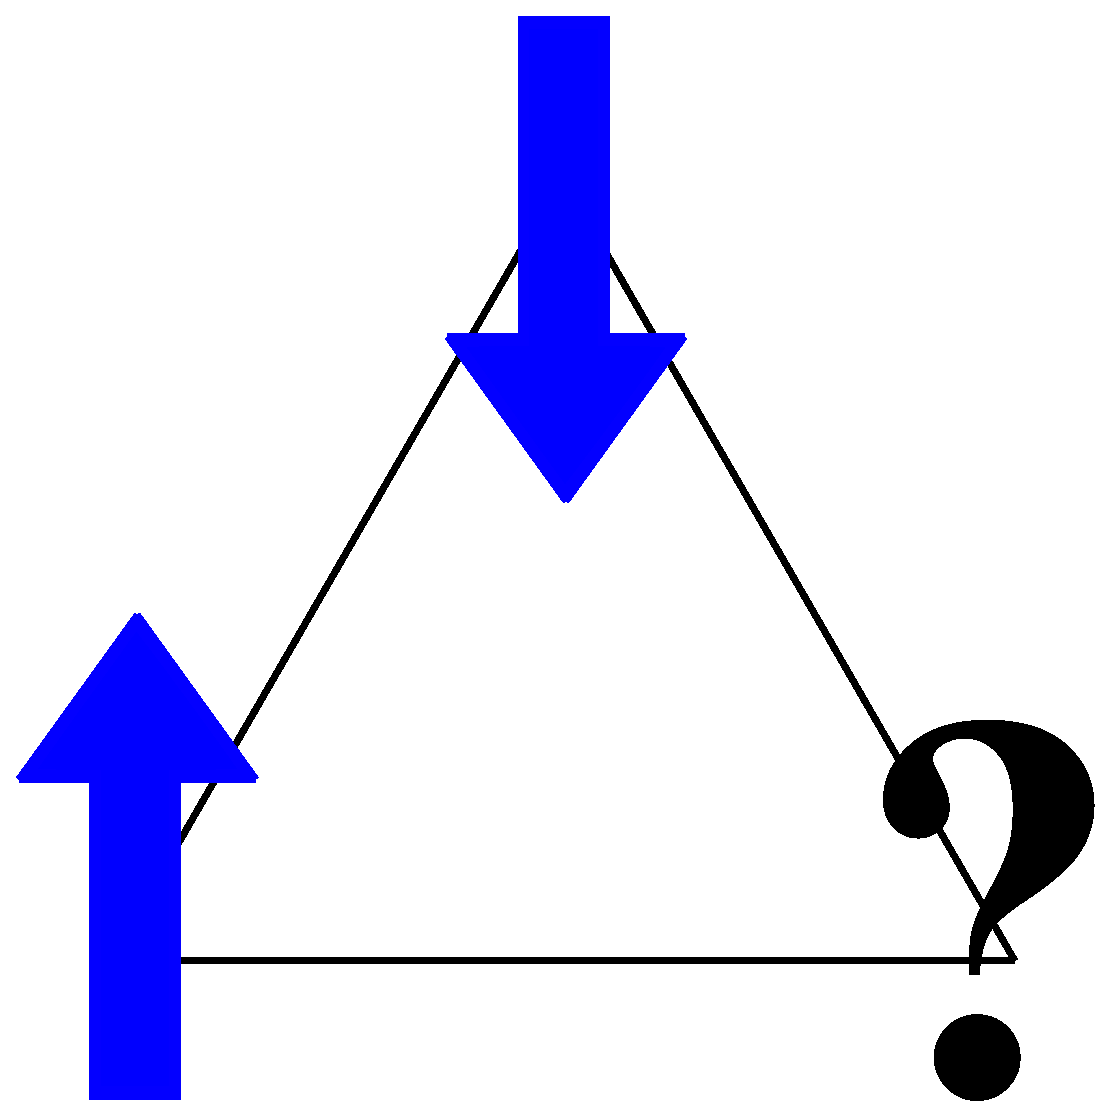
\includegraphics[width=0.5\linewidth]{part1/frust_triangle.eps} \\ а)}
 	\end{minipage}
 	\hfill
 	\begin{minipage}[h]{0.49\linewidth}
 		\center{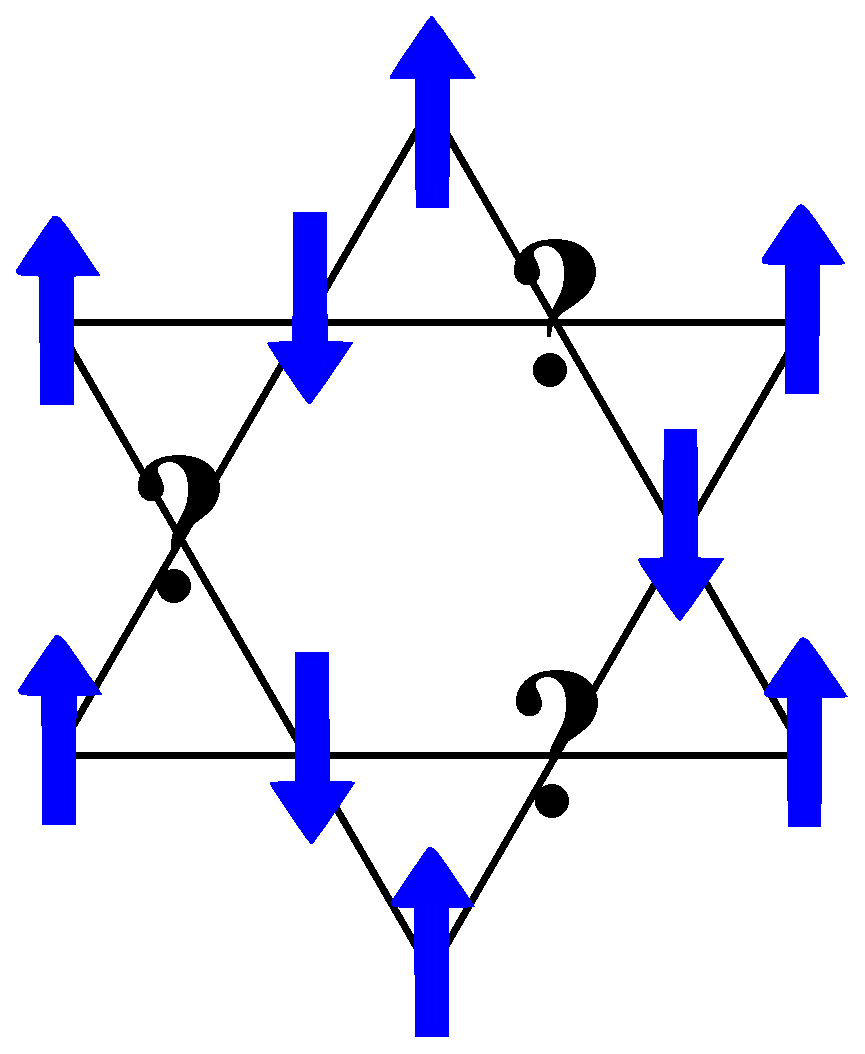
\includegraphics[width=0.5\linewidth]{part1/frust_kagome.eps} \\ б)}
 	\end{minipage}
 	\caption{а) Фрустрация на примере треугольной решетки, б) фрустрация на примере решетки кагоме}
 	\label{frust1}
 \end{figure}

Первым кто обратил внимание на наличие особенностей теплоемкости в антиферромагнитной модели Изинга на треугольной решетке был Ваннье~\cite{wannier1950}, который получил отсутствие фазового перехода в этой модели, температурную зависимость теплоемкости в виде плавного пика и наличие ненулевого значения нуль-температурной энтропии 
\begin{equation}
S_{T\rightarrow 0} = \frac{2}{\pi} \int_{0}^{\pi/3} \ln (2 \cos \omega) d\omega = 0.323066\dots
\label{wannier}
\end{equation}

Таким образом, в такой модели невозможно расположить все спины так, чтобы каждая пара соседей была антипараллельна (рисунок \ref{frust1}а). Фактически, это было первое проявление фрустрации. Причем этот термин был введен только спустя 27 лет после работы Ваннье в статье Жерара Тулуза.


Фрустрации были обнаружены и на других решетках. В частности, при рассмотрении антиферромагнитной модели Изинга на решетке кагоме, точное решение которой было получено Кано и Найя~\cite{kano_naya1953}. В этом случае также невозможно расположить спины так, чтобы каждая пара ближайших соседей была антипараллельна (рисунок \ref{frust1}б). Выражение для нуль-температурной энтропии имеет вид
\begin{multline}
S_{T\rightarrow 0} = \\ = \frac{1}{24\pi^2} \int_{0}^{2\pi} \int_{0}^{2\pi} \ln \{21 - 4 (\cos \omega_1 + \omega_2 + \cos(\omega_1 + \omega_2))\} d\omega_1 d\omega_2 = 0.50183\dots
\end{multline} 

Стоить заметить, что результаты не противоречат третьему началу термодинамики, поскольку энтропия определяется через дифференциал $dS=\delta Q/T$ с точностью до постоянной интегрирования \mbox{$S_0 \geqslant 0$}, и только в формулировке теоремы Нернста – Планка для равновесных систем с невырожденным основным состоянием данная постоянная выбирается нулевой, $S_0 = 0$.

 \begin{figure}[h]
 	\center{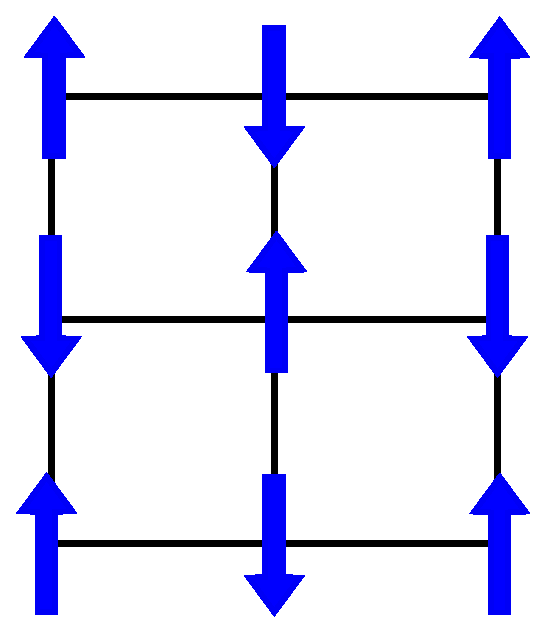
\includegraphics[width=0.3\linewidth]{part1/nofrust_square.eps}}
 	\caption{Антиферромагнитная модель Изинга на квадратной решетке}
 	\label{noFrustSquare}
 \end{figure}

Однако, существуют решетки, которые позволяют расположить спины между собой антипараллельно. Например, к таким относится квадратная решетка~\cite{onsager1941} (рисунок \ref{noFrustSquare}). 

Важно упомянуть, что исследование фрустрационных явлений началось задолго до исследования этого явления на спиновых системах. Так, в 1935 году Полинг \cite{pauling1935} заметил, что атомы водорода в самом обычном водяном льду останутся неупорядоченными даже при абсолютном нуле. То есть даже при охлаждении до нулевой температуры ожидается, что водяной лед будет иметь ненулевую нуль-температурную энтропию, то есть внутреннюю хаотичность. Это связано с тем, что гексагональная кристаллическая структура обычного водяного льда содержит атомы кислорода с четырьмя соседними атомами водорода~(рисунок~\ref{icePyroch}a). Во льду для каждого атома кислорода имеются два соседних атома водорода, находящихся рядом (образуя традиционную молекулу H$_2$O), а два других атома водорода находятся дальше (являясь атомами водорода двух соседних молекул воды). Полинг отметил, что количество конфигураций, соответствующих этому правилу льда «два-близко, два-далеко», растет экспоненциально с увеличением размера системы, и, следовательно, энтропия льда при нулевой температуре должна была быть значительной.

Вместе с тем, к материалам, подверженным фрустрированным взаимодействиям, относится так называемый спиновый лед~\cite{diep2013,bramwell2001,kohli2011,harris1997}. Спиновый лед --- это материал, который состоит из правильных тетраэдров магнитных ионов с угловыми связями, каждый из которых имеет ненулевой магнитный

 \begin{figure}[h]
 	\begin{minipage}[h]{0.49\linewidth}
 		\center{\includegraphics[width=1\linewidth]{part1/waterice.png} \\ а)}
 	\end{minipage}
 	\hfill
 	\begin{minipage}[h]{0.49\linewidth}
 		\center{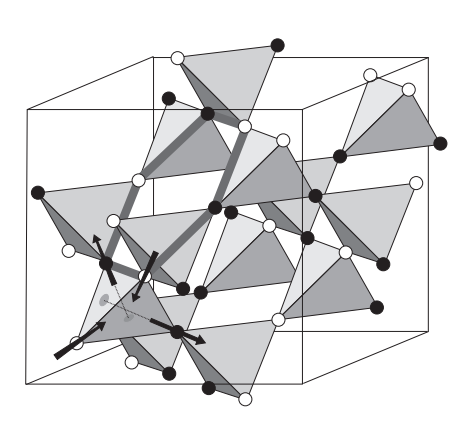
\includegraphics[width=1\linewidth]{part1/pyrochlor.png} \\ б)}
 	\end{minipage}
 	\caption{а) Расположение атомов водорода (черные кружки) вокруг атомов кислорода (белые кружки) во льду, б) Решетка пирохлора, состоящая из тетраэдров с общими углами, занятыми магнитными редкоземельными ионами в материалах спинового льда Ho$_2$Ti$_2$O$_7$ и Dy$_2$Ti$_2$O$_7$~\cite{bramwell2001}}
 	\label{icePyroch}
 \end{figure}

\noindent момент, часто называемый как «спин», который в своем низкоэнергетическом состоянии должен удовлетворять принципу «два-входа---два-выхода» на каждом тетраэдре, образующем кристаллическую структуру~(рисунок~\ref{icePyroch}б). Первыми материалами, идентифицированными как спиновые льды, были пирохлоры Dy$_2$Ti$_2$O$_7$ (титанат диспрозия) и Ho$_2$Ti$_2$O$_7$ (титанат гольмия).

Сделаем важное отступление о том, что при отсутствии фрустрации при заданных параметрах обменных взаимодействий на двумерных решетках мы всегда получаем теплоемкость в виде острого $\Lambda$ - образного пика, при этом имеет место фазовый переход в критической точке~\cite{peierls1936}. А во фрустрированном состоянии всегда имеется пологий куполообразный пик и отсутствие фазового перехода, поскольку основное состояние системы оказывается сильно вырожденным. На рисунке \ref{heatTriangleExpl} приведены графики теплоемкостей модели Изинга на треугольной решетке во фрустрированном и нефрустрированном состояниях.

Здесь и далее, термодинамические и магнитные величины, такие как свободная энергия $F$, энтропия $S$, теплоемкость $C$, намагниченность $M$ и другие, будут изображены на графиках через условные единицы, а именно постоянная Больцмана $k$ будет положена равной единице, а величины $T$ и $H$ будут измеряться в единицах $|J|$, как это принято в теории низкоразмерных систем.

 \begin{figure}[h]
 	\begin{minipage}[h]{0.49\linewidth}
 		\center{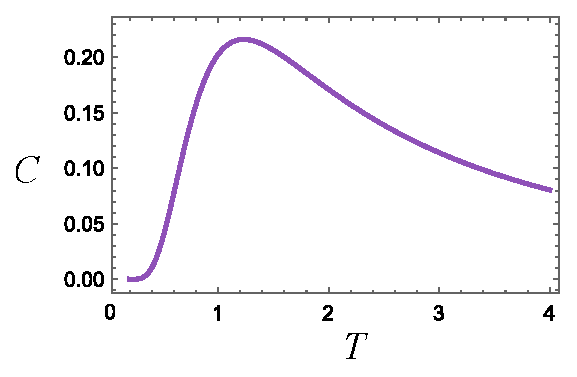
\includegraphics[width=1\linewidth]{part1/heat_triangle_frust.eps} \\ а)}
 	\end{minipage}
 	\hfill
 	\begin{minipage}[h]{0.49\linewidth}
 		\center{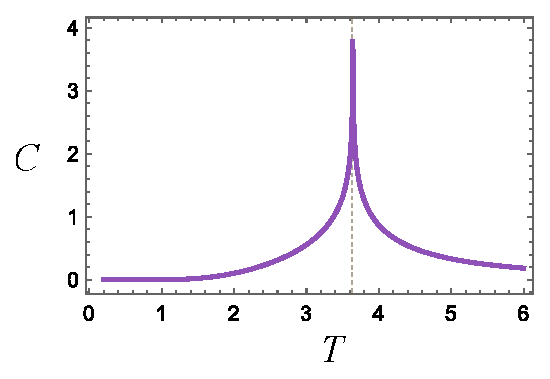
\includegraphics[width=1\linewidth]{part1/heat_triangle_trans.eps} \\ б)}
 	\end{minipage}
 	\caption{Теплоемкость модели Изинга на треугольной решетке: а) система фрустрирована ($J_1 = -1$, $J_2 = -1$, $J_3 = -1$), б) система не фрустрирована ($J_1 = -1$, $J_2 = -1$, $J_3 = 1$). Пунктирной линией обозначена температура фазового перехода}
 	\label{heatTriangleExpl}
 \end{figure}

Материалы спинового льда характеризуются случайным беспорядком в ориентации момента магнитных ионов, даже когда материал находится при очень низких температурах. Это находится в соответствии со случаем водяного льда. Об этом может свидетельствовать широкий гладкий пик теплоемкости, при котором, как уже известно, не возникает фазового перехода и наличие ненулевого значения нуль-температурной энтропии~(рисунок~\ref{HeatAndEntropyExpl}). 

 \begin{figure}[h]
 	\begin{minipage}[h]{0.49\linewidth}
 		\center{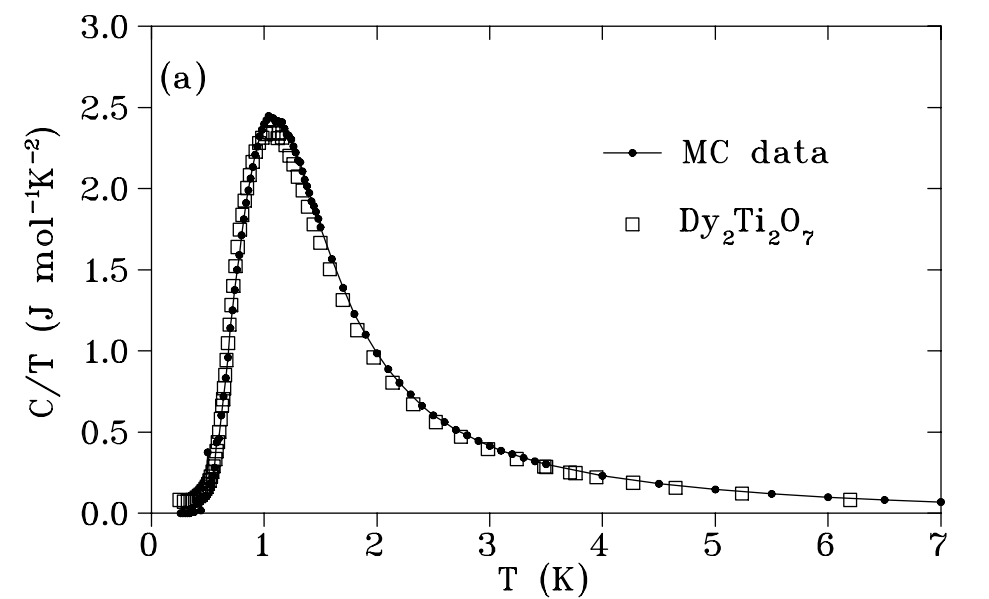
\includegraphics[width=1\linewidth]{part1/heatExpl.png} \\ а)}
 	\end{minipage}
 	\hfill
 	\begin{minipage}[h]{0.49\linewidth}
 		\center{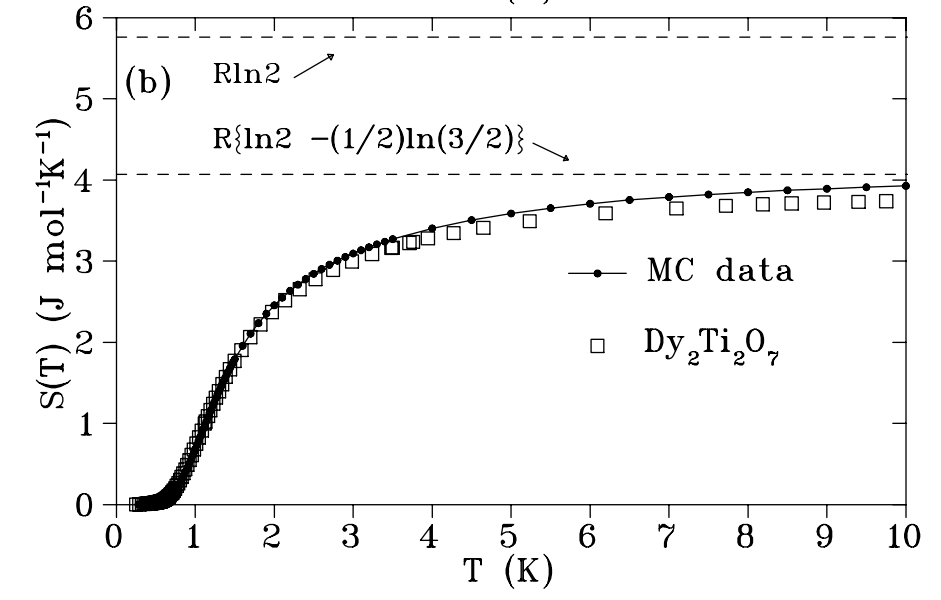
\includegraphics[width=1\linewidth]{part1/entExpl.png} \\ б)}
 	\end{minipage}
 	\caption{а) Теплоемкость и б) энтропия материала спинового льда Dy$_2$Ti$_2$O$_7$ в сравнении с результатами метода Монте-Карло, примененного для модели дипольного спинового льда~\cite{bramwell2001}}
 	\label{HeatAndEntropyExpl}
 \end{figure}

Однако, среди многих типов магнитоупорядоченных веществ особое место принадлежит так называемым спиновым стеклам~\cite{diep2013,docenko1993}.  Обоснованием этого термина служит тот факт, что ориентация элементарных магнитных моментов атомов спинового стекла в области температур ниже некоторой величины $T_{\text{freeze}}$ не имеет никакой пространственной периодичности. В
отличие от парамагнетиков, где элементарные магнитные моменты флуктуируют во времени, спиновые стекла характеризуются наличием «замороженных» магнитных моментов~(рисунок~\ref{SpinGlass}).

 \begin{figure}[b]
 	\center{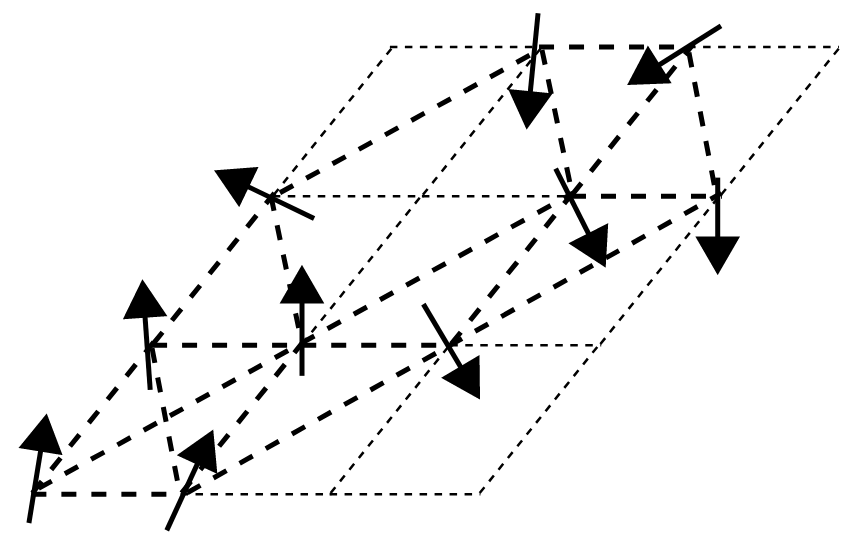
\includegraphics[width=0.5\linewidth]{part1/spinGlass.png}}
 	\caption{Схематическое представление случайной спиновой структуры --- спинового стекла}
 	\label{SpinGlass}
 \end{figure}

Типичные спиновые стекла представляют собой разбавленные магнитные сплавы Cu-Mn, Ag-Mn или Au-Fe, в которых магнитные моменты 3d-элементов взаимодействуют через дальнодействующее обменное взаимодействие. 

Для спиновых стекол характерно, что магнитный момент, наведенный в спиновом стекле внешним магнитным полем, зависит не только от величины поля, но также от предыстории образца. Кроме этого, отличительной чертой поведения спинового стекла является наличие резкого излома на температурной зависимости магнитной восприимчивости, измеренной при малых магнитных полях, а также линейная зависимость теплоемкости от температуры, что говорит о том, что основное состояние спинного стекла сильно вырожденно. 

Считается, что изучение спиновых стекол будет способствовать созданию более совершенных принципов компьютерной памяти. Зависимость магнитного состояния спинового стекла от его магнитной предыстории может использоваться для создания новых материалов магнитной памяти. Также, модель спинового стекла весьма полезна для понимания поведения определенных нейронных сетей, в особенности сетей Хопфилда (искусственная нейронная сеть, в которой каждый нейрон может принимать одно из двух состояний $\pm 1$)~\cite{aarts2001, kincel1987}. 

На одномерной изинговской решетке также наблюдаются фрустрации~\cite{zarubin2019}. Модель Изинга со спином $s = 1$ на одномерной решетке с учетом антиферромагнитного взаимодействия только между ближайшими соседями во внешнем магнитном поле является простейшей моделью, в которой можно обнаружить фрустрации. Ее наибольшее собственное значения уже было найдено в прошлом пункте и оно имеет вид:
\begin{equation}
\lambda_{\text{max}}= e^{\frac{J}{T}}\ch \bigg(\frac{H}{T}\bigg) + \sqrt{e^{\frac{2J}{T}}\ch^2 \bigg(\frac{H}{T}\bigg)-2\sh \bigg(\frac{2J}{T}\bigg)}.
\end{equation}

При $H=0, T=0$ система находится в основном состоянии, представляющее собой антиферромагнитное упорядочение ($\downarrow \uparrow$, где $\downarrow$ --- спин направлен против магнитного поля, $\uparrow$ --- совпадает с направлением поля). С увеличением поля спины начнут выстраиваться вдоль магнитного поля, тем самым возникает ферромагнитная структура ($\uparrow \uparrow$). Можно показать, что в некотором поле, называемом фрустрирующим $H_{\text{fr}}$, энергии этих двух состояний совпадают, и имеется бесконечное количество различных конфигураций с одинаковой энергией. На рисунке \ref{antiferro} показан этот механизм.

 \begin{figure}[h]
 	\center{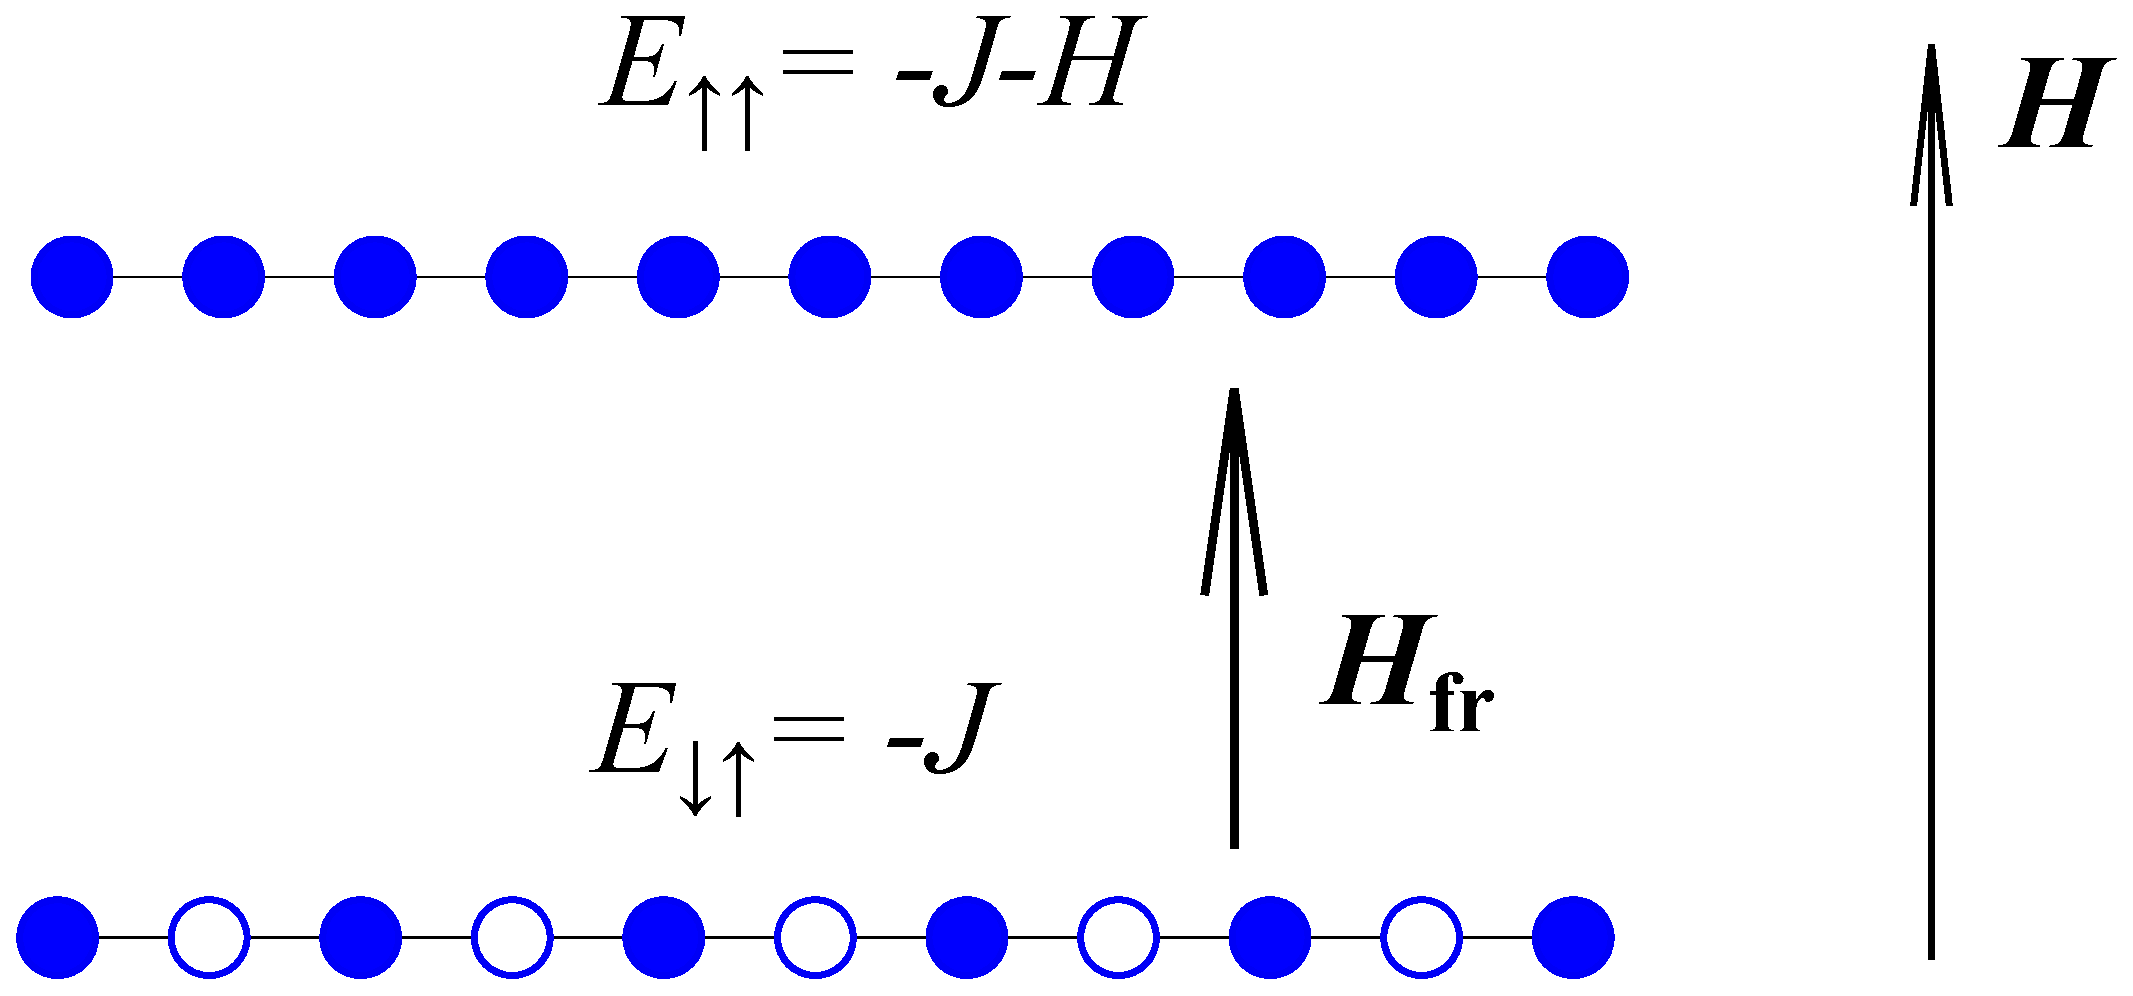
\includegraphics[width=0.65\linewidth]{part1/antiferro.eps}}
 	\caption{Конфигурации, возникающие в модели Изинга при учете ближайших соседей в магнитном поле, для каждой конфигурации приведена соответствующая энергия. Закрашенные кружочки --- спин направлен вверх, прозрачные --- вниз}
 	\label{antiferro}
 \end{figure}

Рассчитаем энергию антиферромагнитной структуры. Данное состояние следует назвать структурой с удвоением периода трансляций решетки, так как оно представляет собой последовательность повторяющихся сегментов $\downarrow \uparrow$. Для определения энергии воспользуемся гамильтонианом \eqref{eq:1.2}, при этом достаточно посчитать энергию только для одного сегмента $\downarrow \uparrow$:
\begin{equation}
E_{\downarrow \uparrow}=-J s_{i}s_{i+1}-H s_{i} =\frac{1}{2}\left( \frac{J}{2}+\frac{J}{2}-H+\frac{J}{2}+\frac{J}{2}+H\right)=J.
\label{eq:2.2}
\end{equation}

Получилось, что энергия структуры, приходящаяся на один узел, находящейся в антиферромагнитном состоянии, представляется обменным взаимодействием между соседними узлами решетки.

Следуя тем же путем, можно определить энергию ферромагнитной структуры:
\begin{equation}
E_{\uparrow \uparrow} = -\frac{J}{2}-\frac{J}{2}-H= -J-H.
\label{eq:2.3}
\end{equation}

Приравнивая энергии \eqref{eq:2.2} и \eqref{eq:2.3} друг к другу, получаем величину фрустрирующего поля для случая взаимодействия только ближайших соседей:
\begin{equation}
H_{\text{fr}}=-2J.
\label{eq:2.4}
\end{equation}

К примеру, при $J=-1$ (антиферромагнитное упорядочивание), имеется фрустрирующее поле $H_{\text{fr}}=2$.

C помощью формул \eqref{eq:1.15} и \eqref{eq:1.17} можно показать, что в точке фрустрации при $T\rightarrow 0$ энтропия равна натуральному логарифму золотого сечения $S=\ln \left[\left(1+\sqrt{5}\right)\!/2\right]$, а намагниченность --- $M=1/\sqrt{5}$.

 \begin{figure}[h]
 	\begin{minipage}[h]{0.49\linewidth}
 		\center{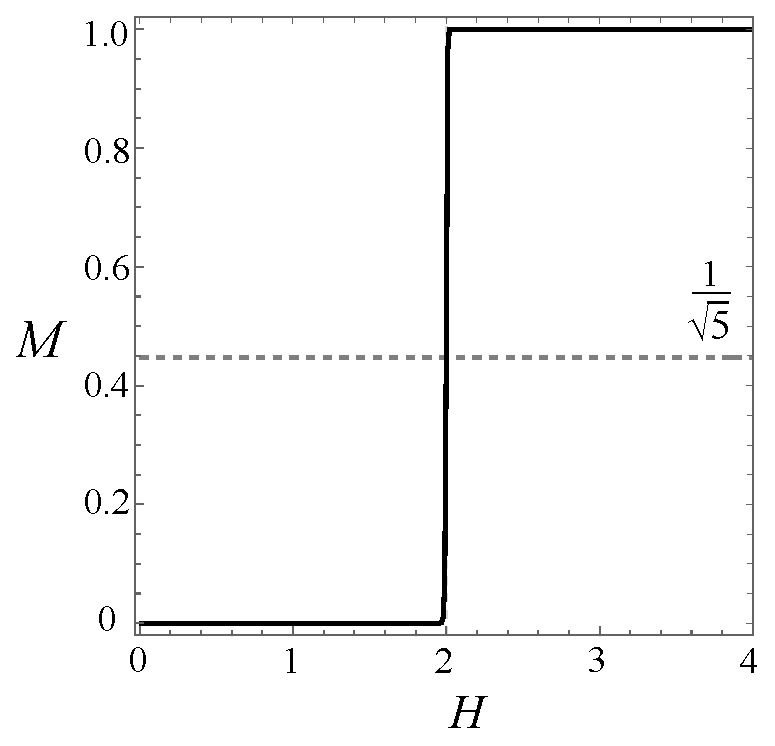
\includegraphics[width=1\linewidth]{part1/magFrust1.eps} \\ а)}
 	\end{minipage}
 	\hfill
 	\begin{minipage}[h]{0.49\linewidth}
 		\center{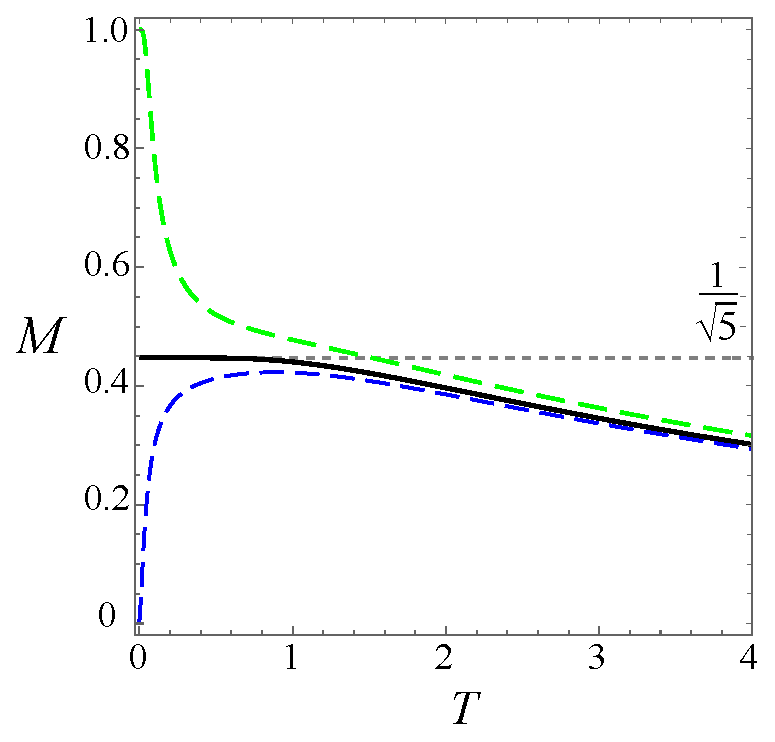
\includegraphics[width=1\linewidth]{part1/magFrust2.eps} \\ б)}
 	\end{minipage}
 	\caption{а) Намагниченность как функция магнитного поля при $T\rightarrow 0$ и б) как функция температуры во фрустрирующем поле при $H_{\text{fr}}=2$ (сплошная линия), при $H_{\text{fr}}=1.95$ (синяя пунктирная линия) и при $H_{\text{fr}}=2.05$ (зеленая пунктирная линия)}
 	\label{magFrust}
 \end{figure}

Итак, рассматривая систему при стремлении температуры к нулю, ее намагниченность испытывает скачок во фрустрирующем поле, таким образом, совершается переход между двумя определенными конфигурациями (рисунок \ref{magFrust}).

В точке фрустрации, с соответствующей нуль-температурной энтропией (рисунок \ref{EntHeatFrust}а), не равной нулю, помимо сходящихся фаз (структур с определенными трансляциями) наблюдается также и бесконечное множество конфигураций, в том числе и без какой-либо трансляционной инвариантности с одинаковой энергией и все вместе они сосуществуют. Однако, если отойти от фрустрации на малую величину магнитного поля (или обменного взаимодействия), то реализуется переход системы в одну какую-то конкретную фазу. Тем самым, система становится упорядоченной, а энтропия стремится к нулю.

 \begin{figure}[h]
 	\begin{minipage}[h]{0.49\linewidth}
 		\center{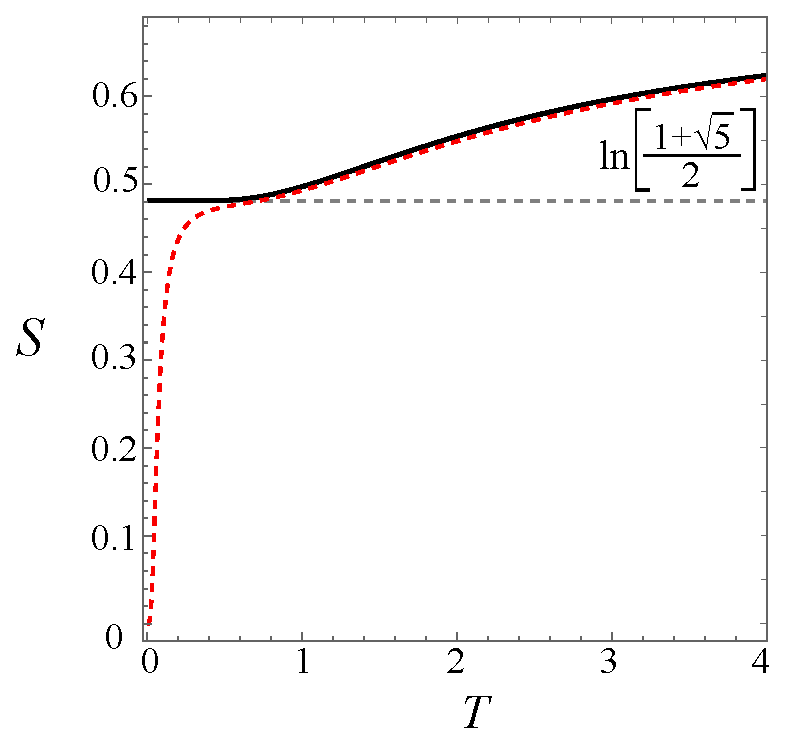
\includegraphics[width=1\linewidth]{part1/entropyFrust.eps} \\ а)}
 	\end{minipage}
 	\hfill
 	\begin{minipage}[h]{0.49\linewidth}
 		\center{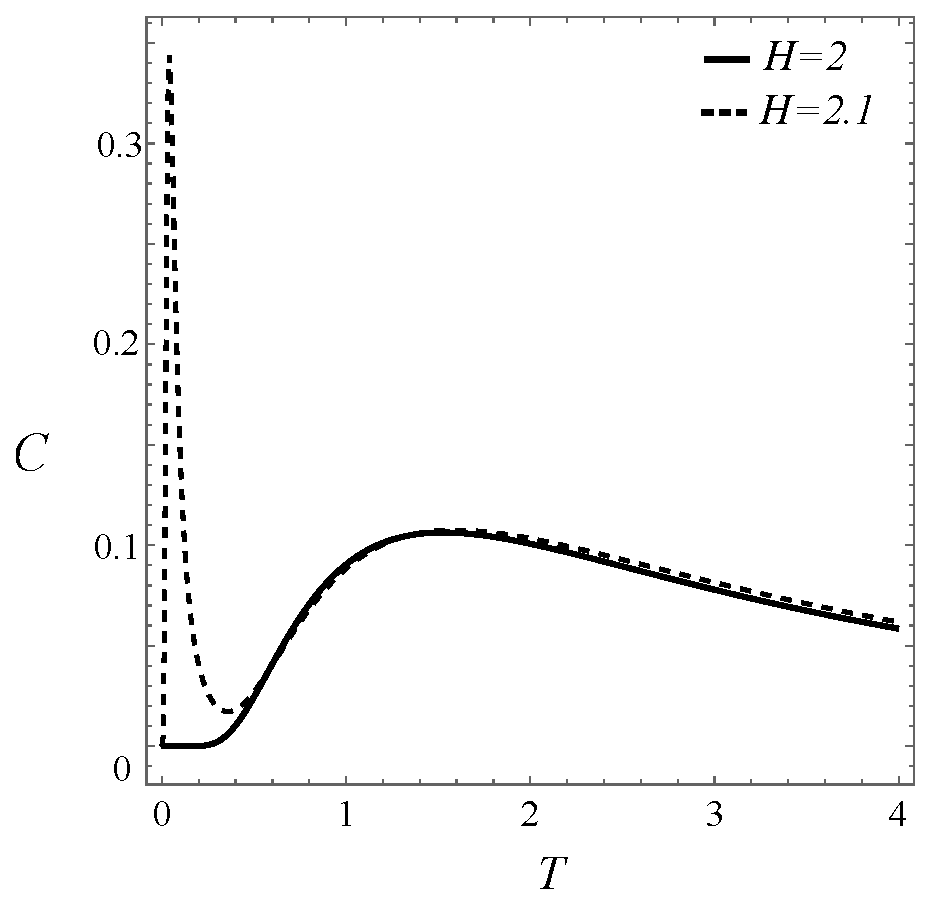
\includegraphics[width=1\linewidth]{part1/heatFrust.eps} \\ б)}
 	\end{minipage}
 	\caption{а) Энтропия во фрустрирующем магнитном поле модели Изинга при учете взаимодействия между ближайшими соседями (сплошная линия). Красной пунктирной линией показана энтропия системы вблизи фрустрации и б) Расщепление теплоемкости около фрустрирующего поля в модели Изинга}
 	\label{EntHeatFrust}
 \end{figure}

Теплоемкость же в непосредственной близости к фрустрации имеет два пика --- острый и широкий плавный~(рисунок~\ref{EntHeatFrust}б). Последний, к тому же, всегда находится правее (в стороне больших температур). Данный факт подтвержден экспериментально~\cite{matsumura1997} (около фрустрирующего поля происходит расщепление теплоемкости на два пика, см. рисунок~\ref{new1}). 

В заключение, стоит отметить любопытное предположение, выдвинутое нами в  статье~[A2] о качественном совпадении явления фрустрации с явлением критической опалесценции. Так как в местах схождения сразу нескольких фаз, фазы не индивидуализированы, а существенно фрустрированы так как, кроме сходящихся фаз, в точках фрустраций существует бесконечное множество конфигураций без каких-либо трансляционных инвариантностей, чему свидетельствует ненулевая нуль-температурная энтропия. А в работе Смолуховского~\cite{smoluchowski1907} установлено, что явление критической опалесценции обусловлено возникновением в тройной точке бесконечного множества термодинамических флуктуаций, поэтому фактически можно сказать, что в тройной точке возникает явление сильных фрустраций.

 \begin{figure}[h]
 	\center{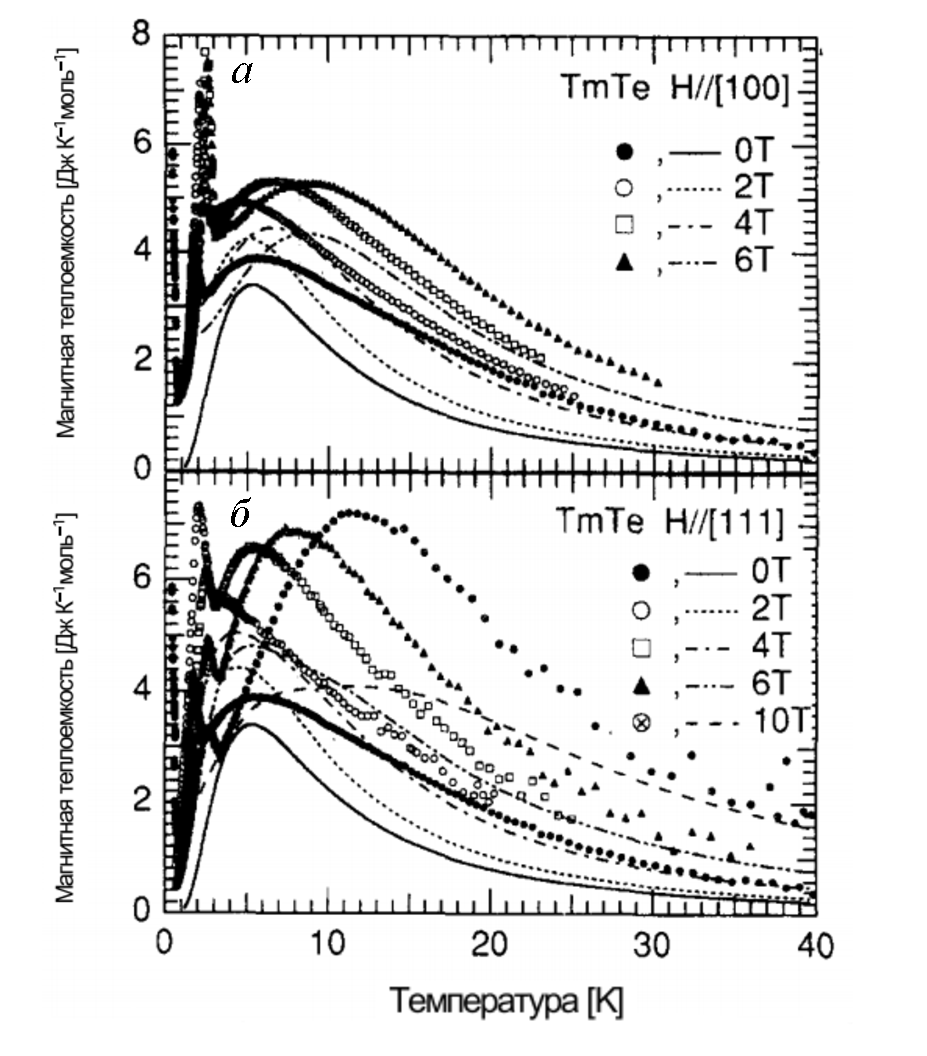
\includegraphics[width=0.6\linewidth]{part1/heatPeakExpl.eps}}
 	\caption{Магнитная теплоемкость TmTe для двух направлений внешнего поля а) [100] и б) [111]~\cite{matsumura1997}}
 	\label{new1}
 \end{figure}

\section{Комбинаторный метод Вдовиченко--Фейнмана}\label{sec:markup}

Идея комбинаторного решения модели Изинга на двумерной решетке принадлежит Фейнману. Суть метода заключается в подсчете всех суперпозиций замкнутых многоугольников (не имеющих общих сторон) на двумерной решетке. Впоследствие, предположение Фейнмана развивалось в статьях Каца и Уорда~\cite{kac1952}, Монтролла~\cite{montroll1953} и Вдовиченко~\cite{vdovichenko1965_1}. Так или иначе, метод берет свое начало с высокотемпературного разложения статистической суммы двумерной решетки. 

Рассмотрим квадратную решетку с $M$ горизонтальными связями и с $M$ вертикальными связями. В термодинамическом пределе $M \rightarrow \infty$ и $M$ совпадает с количеством узлов в решетке $N$. 

Далее, рассмотрим гамильтониан с разными обменными взаимодействиями: по горизонтальному направлению --- $J$, а по вертикальному направлению --- $J^{'}$.

Тогда для статистической суммы модели при нулевом магнитном поле имеем
\begin{equation}
Z_{N} = \sum_{\{\sigma\}} \exp{\bigg[ K_1 \sum_{(i,j)} \sigma_i \sigma_j + K_2 \sum_{(i,k)} \sigma_i \sigma_k\bigg]},
\end{equation}
где первая сумма идет по спинам в горизонтальном направлении, а вторая сумма по спинам в вертикальном направлении
\begin{equation*}
K_1 = \frac{J}{T}; \;\;\;\;\;\; K_2 = \frac{J^{'}}{T}.
\end{equation*}

Используя тождество
\begin{equation}
\exp{[x\sigma_i \sigma_l]} = \ch x (1 + \sigma_i \sigma_l \th x),
\end{equation}
статистическая сумма может быть переписана в виде
\begin{equation}
Z_{N} = (\ch K_1 \ch K_2)^M \sum_{\{\sigma\}} \prod_{(i,j)} (1 + v \sigma_i \sigma_j) \prod_{(i,k)} (1 + w \sigma_i \sigma_k),
\label{zn1} 
\end{equation}
\begin{equation*}
v = \th K_1; \;\;\;\;\;\; w = \th K_2.
\end{equation*}

Оба параметра $v$ и $w$ всегда меньше 1 для всех значений температуры $T$, кроме $T = 0$, при котором $v = w = 1$. В частности, они являются малыми параметрами в высокотемпературном разложении, поэтому следует искать разложение статсуммы вблизи $T = \infty$.

Если разложить произведение в формуле \eqref{zn1}, получится $2^{2M}$ слагаемых, поскольку имеется $2M$ множителей (по одному на каждый сегмент)
и в каждом из них есть два слагаемых. Можно ввести графическое представление этого разложения. Линия, проведенная между узлами решетки по горизонтали $(i, j)$, соответствует множителю $v \sigma_i \sigma_j$, линия, проведенная между узлами решетки по вертикали  $(i, k)$, соответствует множителю $v \sigma_i \sigma_k$. Отсутствие линии между узлами решетки соответствует множителю 1. Повторяя данную операцию для $2^{2M}$ слагаемых, можно установить соответствие между членами в разложении и графическими конфигурациями. Общее выражении этих слагаемых таково
\begin{equation*}
v^r w^s \sigma_1^{n_1} \sigma_2^{n_2} \sigma_3^{n_3} \dots.
\end{equation*}
где $r$ --- общее число горизонтальных связей, $s$ --- общее число вертикальных связей, $n_i$ --- количество линий, где $i$ --- конечный узел. 

Теперь необходимо посчитать сумму по всем спинам решетки, чтобы получить статсумму. Поскольку каждый спин $\sigma_i$ принимает значения $\pm 1$, получаем нулевую сумму, если все $n_1$, $n_2$, \dots, $n_N$ являются четными и этом случае результат равен $2^N v^r w^s$. Исходя из этих соображений, статистическая сумма может быть выражена как

\begin{equation}
Z_{N} = 2^N (\ch K_1 \ch K_2)^M \sum_{P} v^{r} w^{s}, 
\end{equation}
где сумма идет по всем конфигурациям линий на решетке с четным количеством линий на каждом узле решетки, то есть сумма взята по всем замкнутым многоугольникам $P$ решетки. Таким образом, статсумма, не считая множителя, задается геометрической величиной
\begin{equation}
\Phi(v, w) = \sum_{P} v^r w^s.
\label{phi}
\end{equation}

Вычислить первые члены этой суммы нетрудно. Первый член равен 1 и
соответствует случаю, когда на решетке нет многоугольников. Второй член
соответствует наименьшему замкнутому многоугольнику на решетке, т.е. квадрату с единичной длиной, как показано на рисунке \ref{secondTermExtension}. Количество таких квадратов равно $N$, так как они могут размещаться на любом из $N$ узлов решетки. Каждый из них имеет вес $(vw)^2$, поэтому второй член суммы \eqref{phi} равен $N(vw)^2$. Следующая замкнутая фигура представляет собой прямоугольник из 6 связей, их может быть два вида: $v^4 w^2$ и $v^2 w^4$, как показано на рисунке \ref{thirdTermExtension}. Количество таких прямоугольников также может быть $N$ штук. Используя эти первые члены разложения функции $\Phi(v, w)$ запишем
\begin{equation}
\Phi(v, w) = 1 + N (vw)^2 + N (v^4 w^2 + v^2 w^4) + \dots.
\end{equation}

 \begin{figure}[h]
 	\center{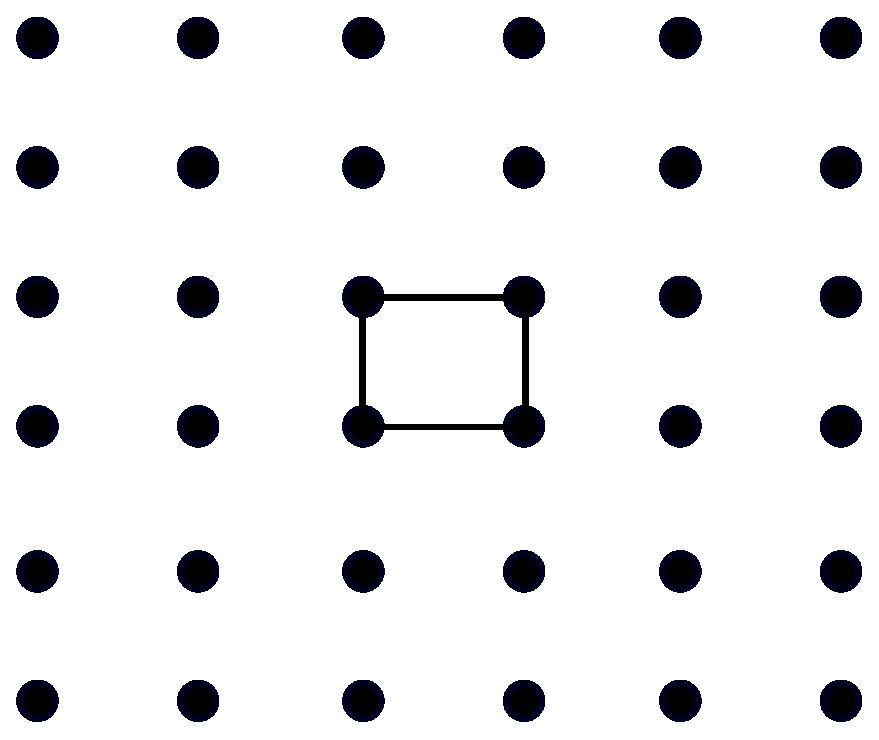
\includegraphics[width=0.4\linewidth]{part1/secTerm.eps}}
 	\caption{Второй член высокотемпературного разложения}
 	\label{secondTermExtension}
 \end{figure} 

 \begin{figure}[h]
 	\center{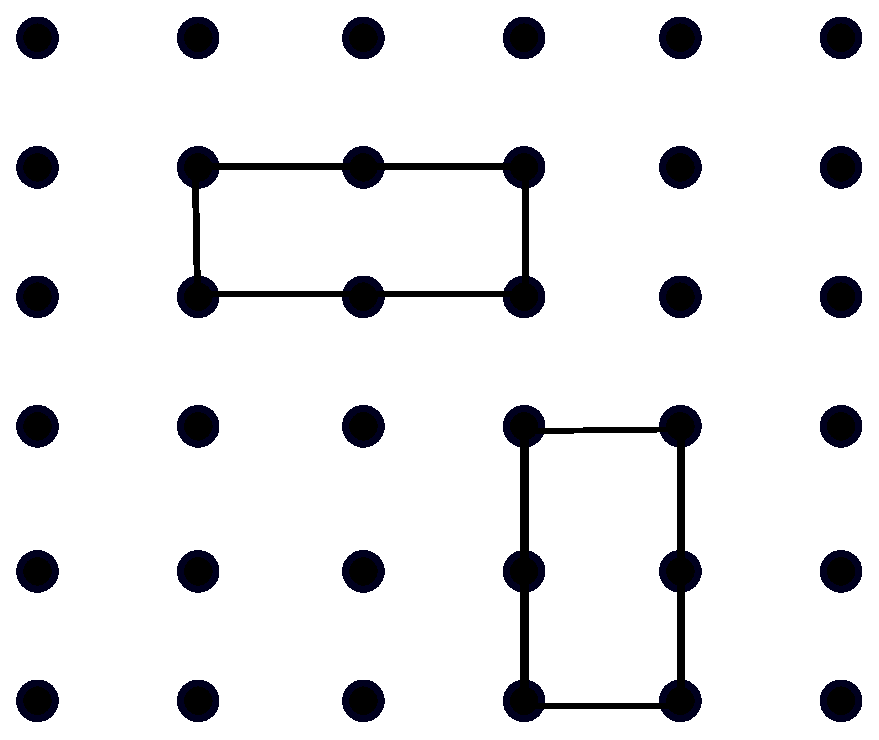
\includegraphics[width=0.4\linewidth]{part1/thirdTerm.eps}}
 	\caption{Третий член высокотемпературного разложения}
 	\label{thirdTermExtension}
 \end{figure} 

Следовательно, для знания статсуммы нужно посчитать все члены в разложении $\Phi(v, w)$, однако вычисление следующих членов $\Phi(v, w)$ стремительно усложняется. 

Изящное решение данной проблемы было предложено Вдовиченко~\cite{vdovichenko1965_1}. Метод решения подразделяется на три шага: (a) первый шаг состоит в выражении суммы по многоугольникам в виде суммы по замкнутым циклам без пересечений; (б) второй шаг заключается в преобразовании суммы по замкнутым циклам без пересечений в сумму по всем возможным замкнутым циклам; (в) на последнем шаге задача сводится к случайному блужданию по решетке.

 \begin{figure}[h]
 	\center{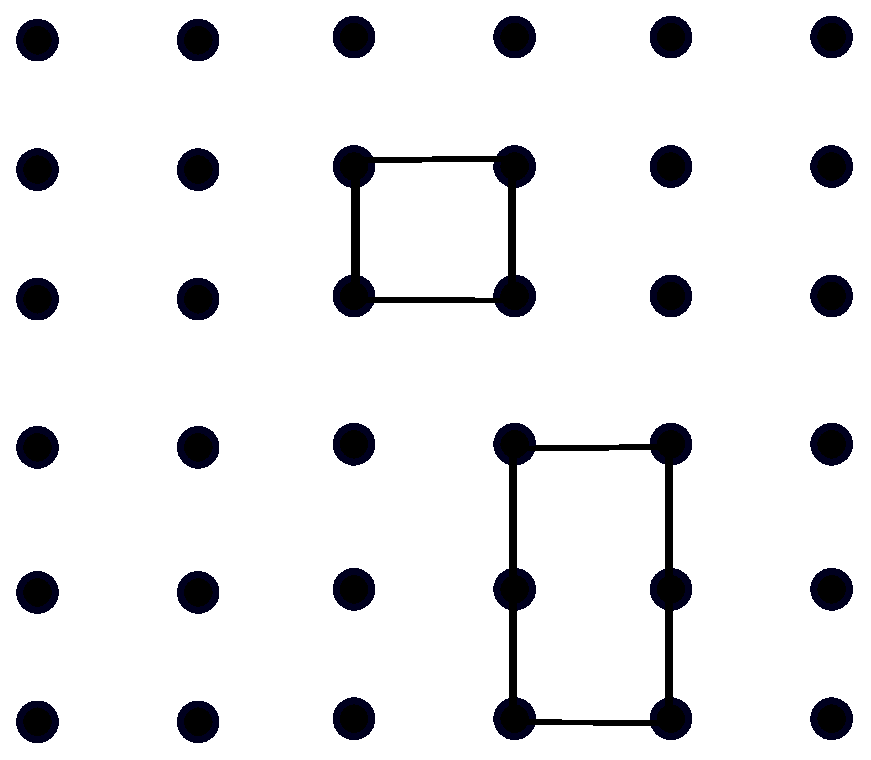
\includegraphics[width=0.4\linewidth]{part1/noIntersectPolygons.eps}}
 	\caption{Непересекающиеся многоугольники}
 	\label{noInterpolygons}
 \end{figure}   

 \begin{figure}[h]
 	\center{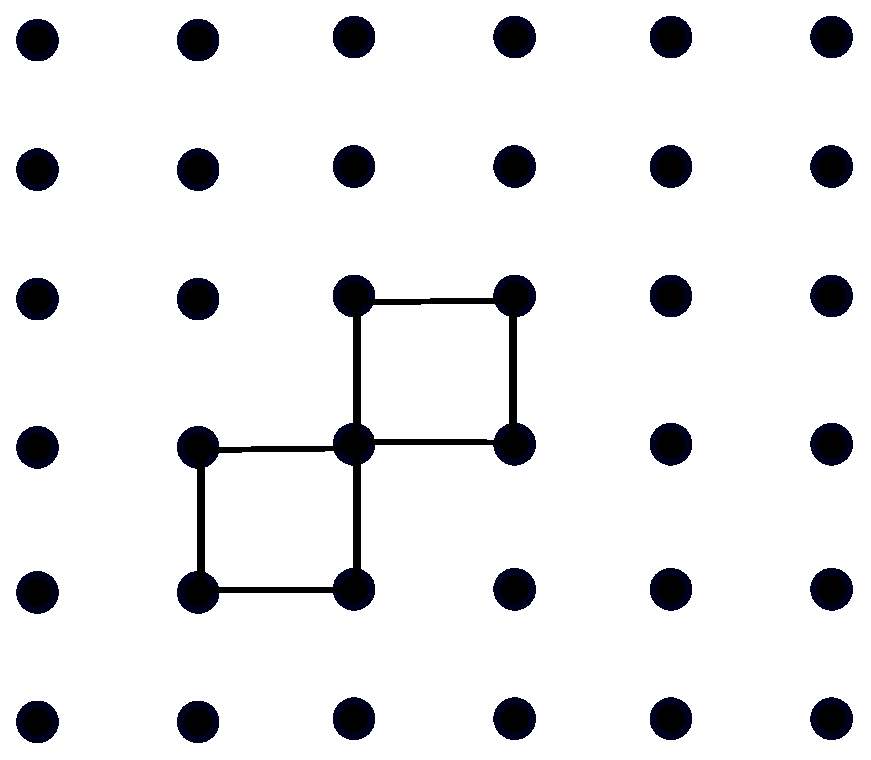
\includegraphics[width=0.4\linewidth]{part1/SelfIntersectPolygons.eps}}
 	\caption{Самопересекающийся многоугольник}
 	\label{selfpolygons}
 \end{figure}  

Обсудим реализацию первого шага, то есть как организовать сумму по многоугольникам с точки зрения их соединенных частей. Заметим, что каждый многоугольник состоит из одной или нескольких связанных частей. Для несамопересекающихся многоугольников это утверждение очевидно: например, многоугольник на рисунке \ref{noInterpolygons} состоит из двух несвязных частей. Но для самопересекающихся многоугольников утверждение может быть неоднозначным, и в зависимости от разложения могут быть разные связанные части. Чтобы прояснить этот вопрос, рассмотрим многоугольник на рисунке \ref{selfpolygons}. Его можно разложить тремя разными способами, как показано на рисунке \ref{threeVarPoly}: его можно разложить на одну или две соединенные части без пересечения или в одну соединенную часть, но с пересечением. Легко показать, что это правило является общим, а именно всегда существует три возможных разложения для всех самопересечений многоугольников. 

 \begin{figure}[h]
 	\center{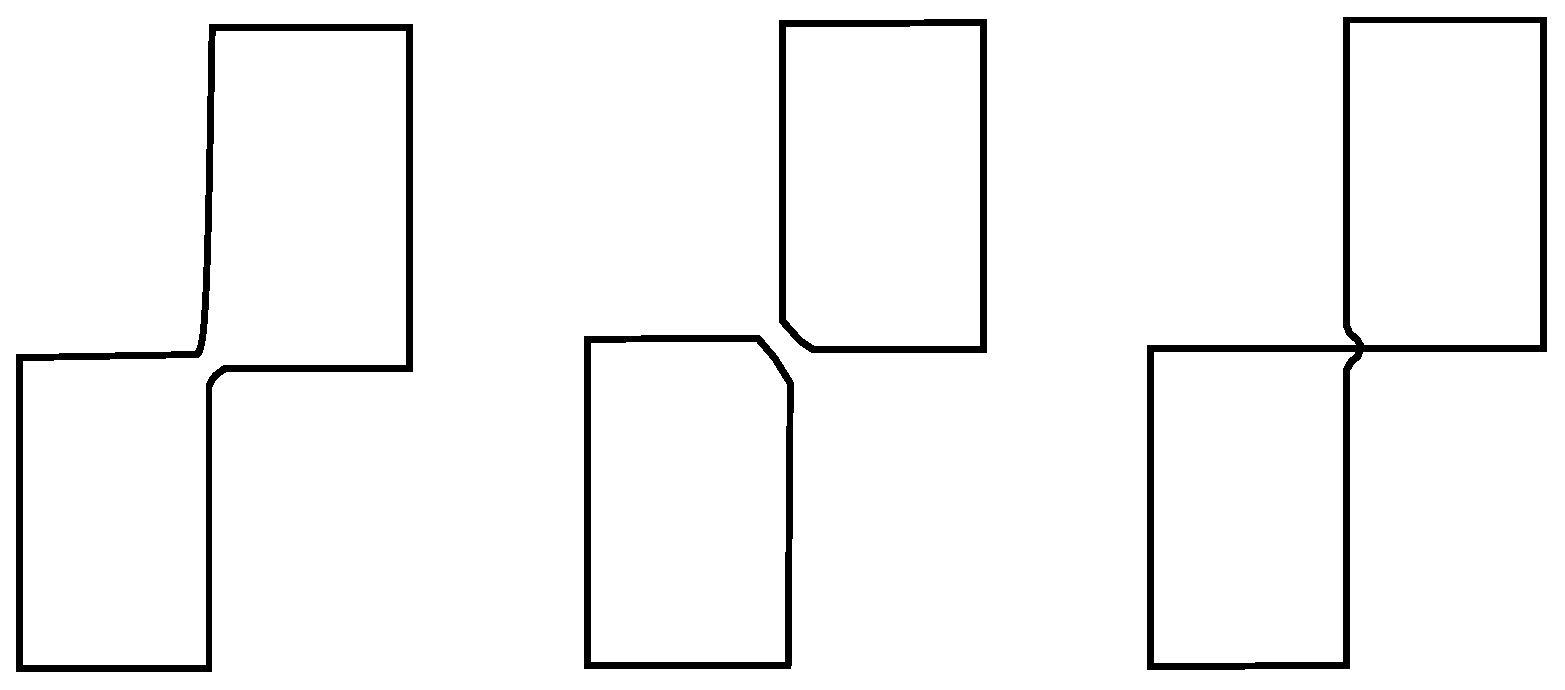
\includegraphics[width=0.5\linewidth]{part1/threeVarPoly.eps}}
 	\caption{Три различных разложения на связные части для самопересекающегося многоугольника}
 	\label{threeVarPoly}
 \end{figure}

 \begin{figure}[h]
 	\center{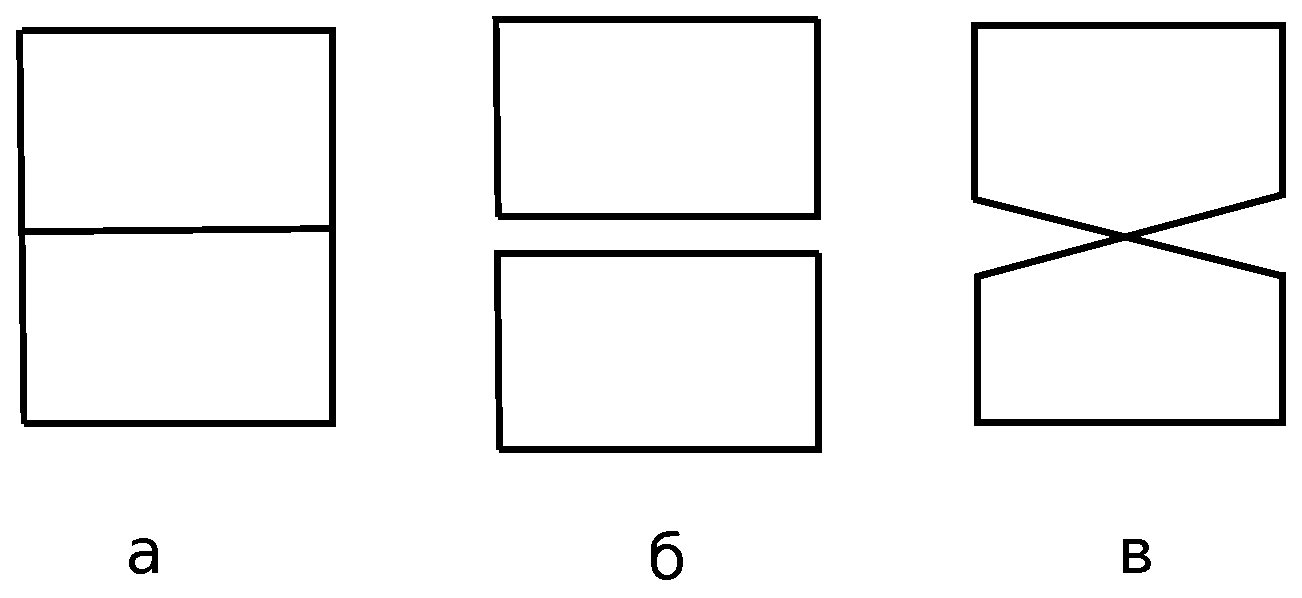
\includegraphics[width=0.5\linewidth]{part1/polyRepeatBonds.eps}}
 	\caption{Многоугольник с повторяющимися связями}
 	\label{PolyRepeatBonds}
 \end{figure}

Сумма по многоугольникам, указанная в уравнении \eqref{phi}, может быть организована в сумму по соединенным частям многоугольников, но нужно действовать осторожно, чтобы правильно подсчитать различные члены разложения, в частности, чтобы не подсчитывать одну и ту же конфигурацию более одного раза. Эта проблема может быть решена путем взвешивания каждого многоугольника с коэффициентом $(-1)^n$, где $n$ - общее количество самопересечений замкнутого многоугольника. Таким образом, все лишние члены в сумме исчезают. В примере на рисунке \ref{threeVarPoly} первые два члена имеют вес $+1$, а последний член $-1$, так что в окончательном выражении сохраняется только один член.

Обратите внимание, что, приняв приведенное выше правило для выполнения суммирования по замкнутым многоугольникам, можно включить в сумму также многоугольники с повторяющимися связями. Простейший из них представлен на рисунке \ref{PolyRepeatBonds}. Эти многоугольники явно отсутствуют в исходной формулировке высокотемпературного разложения, так как на некоторых узлах имеется нечетное количество связей. Однако, учитывая вес связи, легко увидеть, что эти члены в сумме сокращаются.

Однако, по-прежнему существует недостаток в процедуре взвешивания многоугольника, поскольку он зависит от глобального свойства многоугольника, такого как количество его пересечений. Было бы удобнее выразить вес $(−1)^n$ локальным способом. Это возможно благодаря известному геометрическому свойству: общий угол поворота касательной, проходящей вокруг замкнутого плоского контура, равен $2\pi (\xi + 1)$, где $\xi$ - целое число (положительное или отрицательное), с четностью, совпадающей с номером $\nu$ самопересечения замкнутого многоугольника. Следовательно, мы можем присвоить каждой точке замкнутого многоугольника фазовый множитель $e^{i\alpha / 2}$, где угол поворота $\alpha$ принимает значения $\alpha = 0, \pm \pi/ 2$ в соответствии с углом изменения направления на следующую связь, так что произведение всех этих множителей по петле дает $(−1)^{\nu + 1}$. Для набора из $k$ петель имеем $(−1)^{n + k}$, где $n = \sum \nu$.

Таким образом, мы можем автоматически учитывать количество самопересечений многоугольника, взвешивая каждый узел на $e^{i\alpha/2}$ и умножая член, соответствующий данному многоугольнику (заданному набором из $k$ петель), на множитель $(−1)^k$, поскольку этот член будет компенсировать то же слагаемое, что и в предыдущем выражении $(-1)^{n + k}$.

Далее для простоты повествования рассмотрим только изотропный случай квадратной решетки, а именно, когда обменное взаимодействие в горизонтальном и вертикальном направлениях одинаково, так что в статистическую сумму входит только параметр $v = \th K$, где $K = J/T$. Тогда статсумма такой решетки будет даваться выражением
\begin{equation}
Z_N = 2^N \ch^{2N} \!\!K\; \Phi(v),
\label{zn2}
\end{equation}
при
\[ \Phi(v) = \sum_r g_r v^r, \]
где $g_r$ --- количество замкнутых необязательно связанных многоугольников, заданных четным числом $r$ связей.

Обозначим через $f_{r}$ сумму по отдельным замкнутым многоугольникам, состоящих из $r$ звеньев. Каждый многоугольник взвешен в соответствии с указанным выше правилом. Сумма по всем парам многоугольников с общим числом звеньев $r$ определяется выражением
\begin{equation*}
\frac{1}{2!} \sum_{\substack{r_1 + r_2 = r}} f_{r_1} f_{r_2},
\end{equation*}
где множитель $2!$ в знаменателе учитывает, что перестановка двух индексов приводит к одной и той же паре замкнутых многоугольникам. Аналогичный множитель $n!$ присутствует в знаменателе суммы для $n$ многоугольников.

Следовательно, функцию $\Phi$ можно записать как
\begin{equation}
\Phi(v) = \sum_{n = 0} (-1)^n \frac{1}{n!} \sum_{\substack{r_1, r_2, \dots = 1}} v^{r_1 + r_2 + \dots + r_n} f_{r_1} \dots f_{r_n}.
\end{equation}

Поскольку в $\Phi$ есть члены, соответствующие множествам петель с любой возможной общей длиной $r = r_1 + r_2 + \dots$, в сумме  индексы $r_1, r_2, \dots$ принимают независимо все значения от $1$ до $\infty$, так что
\begin{equation*}
\sum_{\substack{r_1, r_2, \dots}} v^{r_1 + r_2 + \dots + r_n} f_{r_1} \dots f_{r_n} = \bigg(\sum_{r=1}^{\infty}v^r f_{r}\bigg)^n.
\end{equation*}

Таким образом, $\Phi$ выражается как
\begin{equation}
\Phi (v) = \exp{\bigg[-\sum_{r=1}^{\infty}v^r f_{r}\bigg]}.
\label{Phi}
\end{equation}

Этим выражением завершаются шаги (а) и (б) метода Вдовиченко.
Остается только явно вычислить величину $f_{r}$.

 \begin{figure}[h]
 	\center{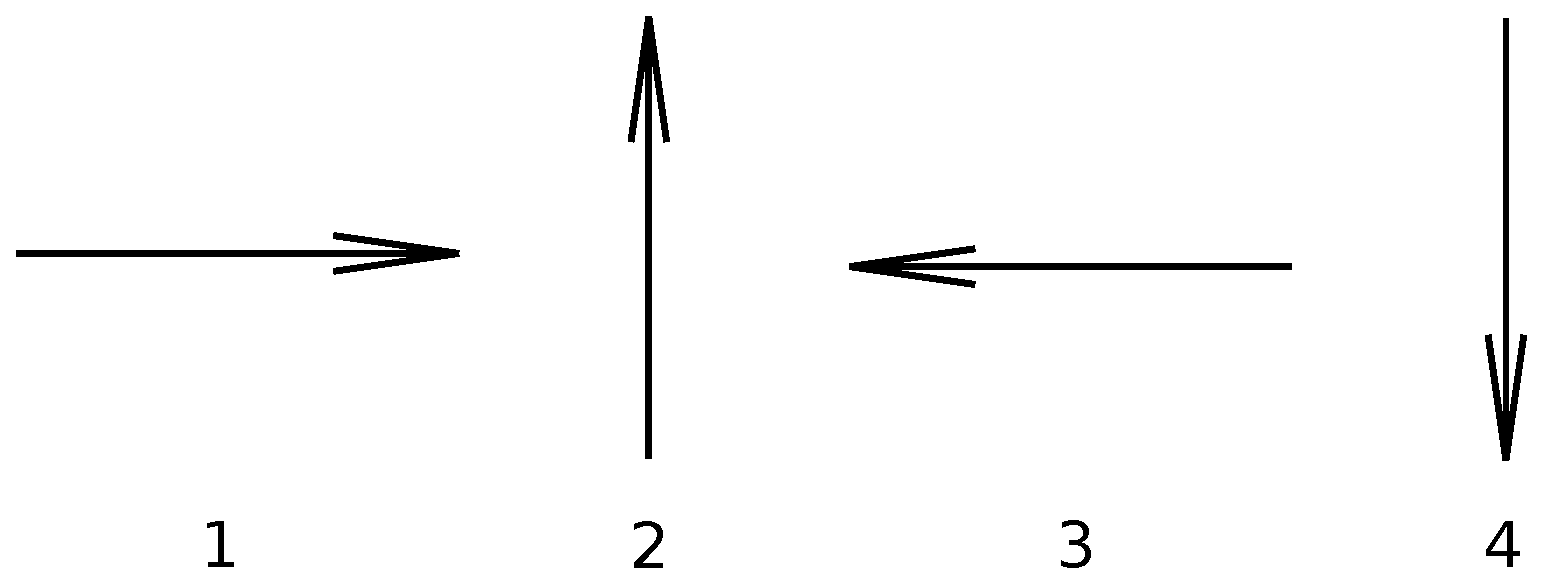
\includegraphics[width=0.5\linewidth]{part1/dirSquare.eps}}
 	\caption{Возможные направления движения по квадратной решетке}
 	\label{dirSquare}
 \end{figure}

Поскольку на квадратной решетке есть четыре различных направления, по которым можно передвигаться, то их удобно пронумеровать индексом $\mu = 1, 2, 3, 4$, как показано на рисунке \ref{dirSquare}. Введем новую функцию $W_r (i, j, \mu)$, которая определяется как сумма по всем возможным путям длины $r$, начинающиеся из заданной точки с координатами $(i_0, j_0)$ вдоль направления $\mu_0$ и достигая в точке координаты $(i, j)$ вдоль направления $\mu$. Пути, входящие в определение $W_r (i, j, \mu)$, взвешиваются с учетом ранее введенных множителей $e^{i\alpha / 2}$. Если теперь выбрать $(i_0, j_0)$ в качестве начальной точки, $W_r (i_0, j_0, \mu_0)$ станет суммой по всем многоугольникам, выходящим и возвращающимся в ту же точку. В результате, имеем тождество
\begin{equation}
f_{r} = \frac{1}{2r} \sum_{i_0, j_0, \mu} W_r (i_0, j_0, \mu),
\label{fl}
\end{equation}
где член $1 / (2r)$ учитывает тот факт, что в сумме в правой части каждый замкнутый многоугольник может быть пересечен в двух противоположных направлениях и может иметь любой из своих $r$ узлов в качестве отправной точки. Благодаря своему определению, функция $W_r (i, j, \mu)$ удовлетворяет рекурсивным уравнениям
\begin{align}
&W_{r+1} (i, j, 1) = W_r (i − 1, j, 1) + e^{−i \frac{\pi}{4}} W_r (i, j − 1, 2) + 0 + e^{i \frac{\pi}{4}} W_r (i, j + 1, 4), \nonumber \\
&W_{r+1} (i, j, 2) = e^{i \frac{\pi}{4}} W_r (i − 1, j, 1) + W_r (i, j − 1, 2) + e^{−i \frac{\pi}{4}} W_r (i + 1, j, 3) + 0, \nonumber\\
& W_{r+1} (i, j, 3) = 0 + e^{−i \frac{\pi}{4}} W_r (i, j − 1, 2) + W_r (i + 1, j, 3) + e^{-i\frac{\pi}{4}} W_r (i, j + 1, 4), \nonumber\\
& W_{r+1} (i, j, 4) = e^{−i \frac{\pi}{4}} W_r (i − 1, j, 1) + 0 + e^{i \frac{\pi}{4}} W_r (i + 1, j, 3) + W_r (i, j + 1, 4).
\label{eq}
\end{align}

Рассмотрим, например, первое уравнение \eqref{eq}. В точку $i$, $j$, $1$ можно попасть, сделав последний $(r + 1)$-й шаг слева, снизу или сверху, но не справа. Коэффициенты, представленные в уравнении, основаны на фазовых факторах, относящихся к изменению направлений. Используя те же аргументы, можно вывести другие уравнения в \eqref{eq}. Вводя матрицу коэффициентов $\Lambda$, рекурсивные уравнения можно записать в виде
\begin{equation}
W_{r+1}(i, j, \mu) = \sum_{i^{'},\; j^{'},\; \mu^{'}} \Lambda (ij\mu\; |\; i^{'}j^{'}\mu^{'}) W_{r} (i^{'}, j^{'}, \mu^{'}),
\end{equation}
которые допускают наводящую на размышления интерпретацию: эти уравнения можно интерпретировать как марковский процесс, связанный со случайным блужданием по решетке, с вероятностью перехода между двумя ближайшими соседними узлами, выраженными относительным матричным элементом $\Lambda$. Поскольку существует четыре возможных направления для этого движения, при сохранении всех остальных параметров фиксированными, $\Lambda$ представляет собой матрицу $4 \times 4$ с индексами $\mu^{'}$ и $\mu$, графическая интерпретация которой показана на рисунке \ref{matrixElemSquare}.

 \begin{figure}[h]
 	\center{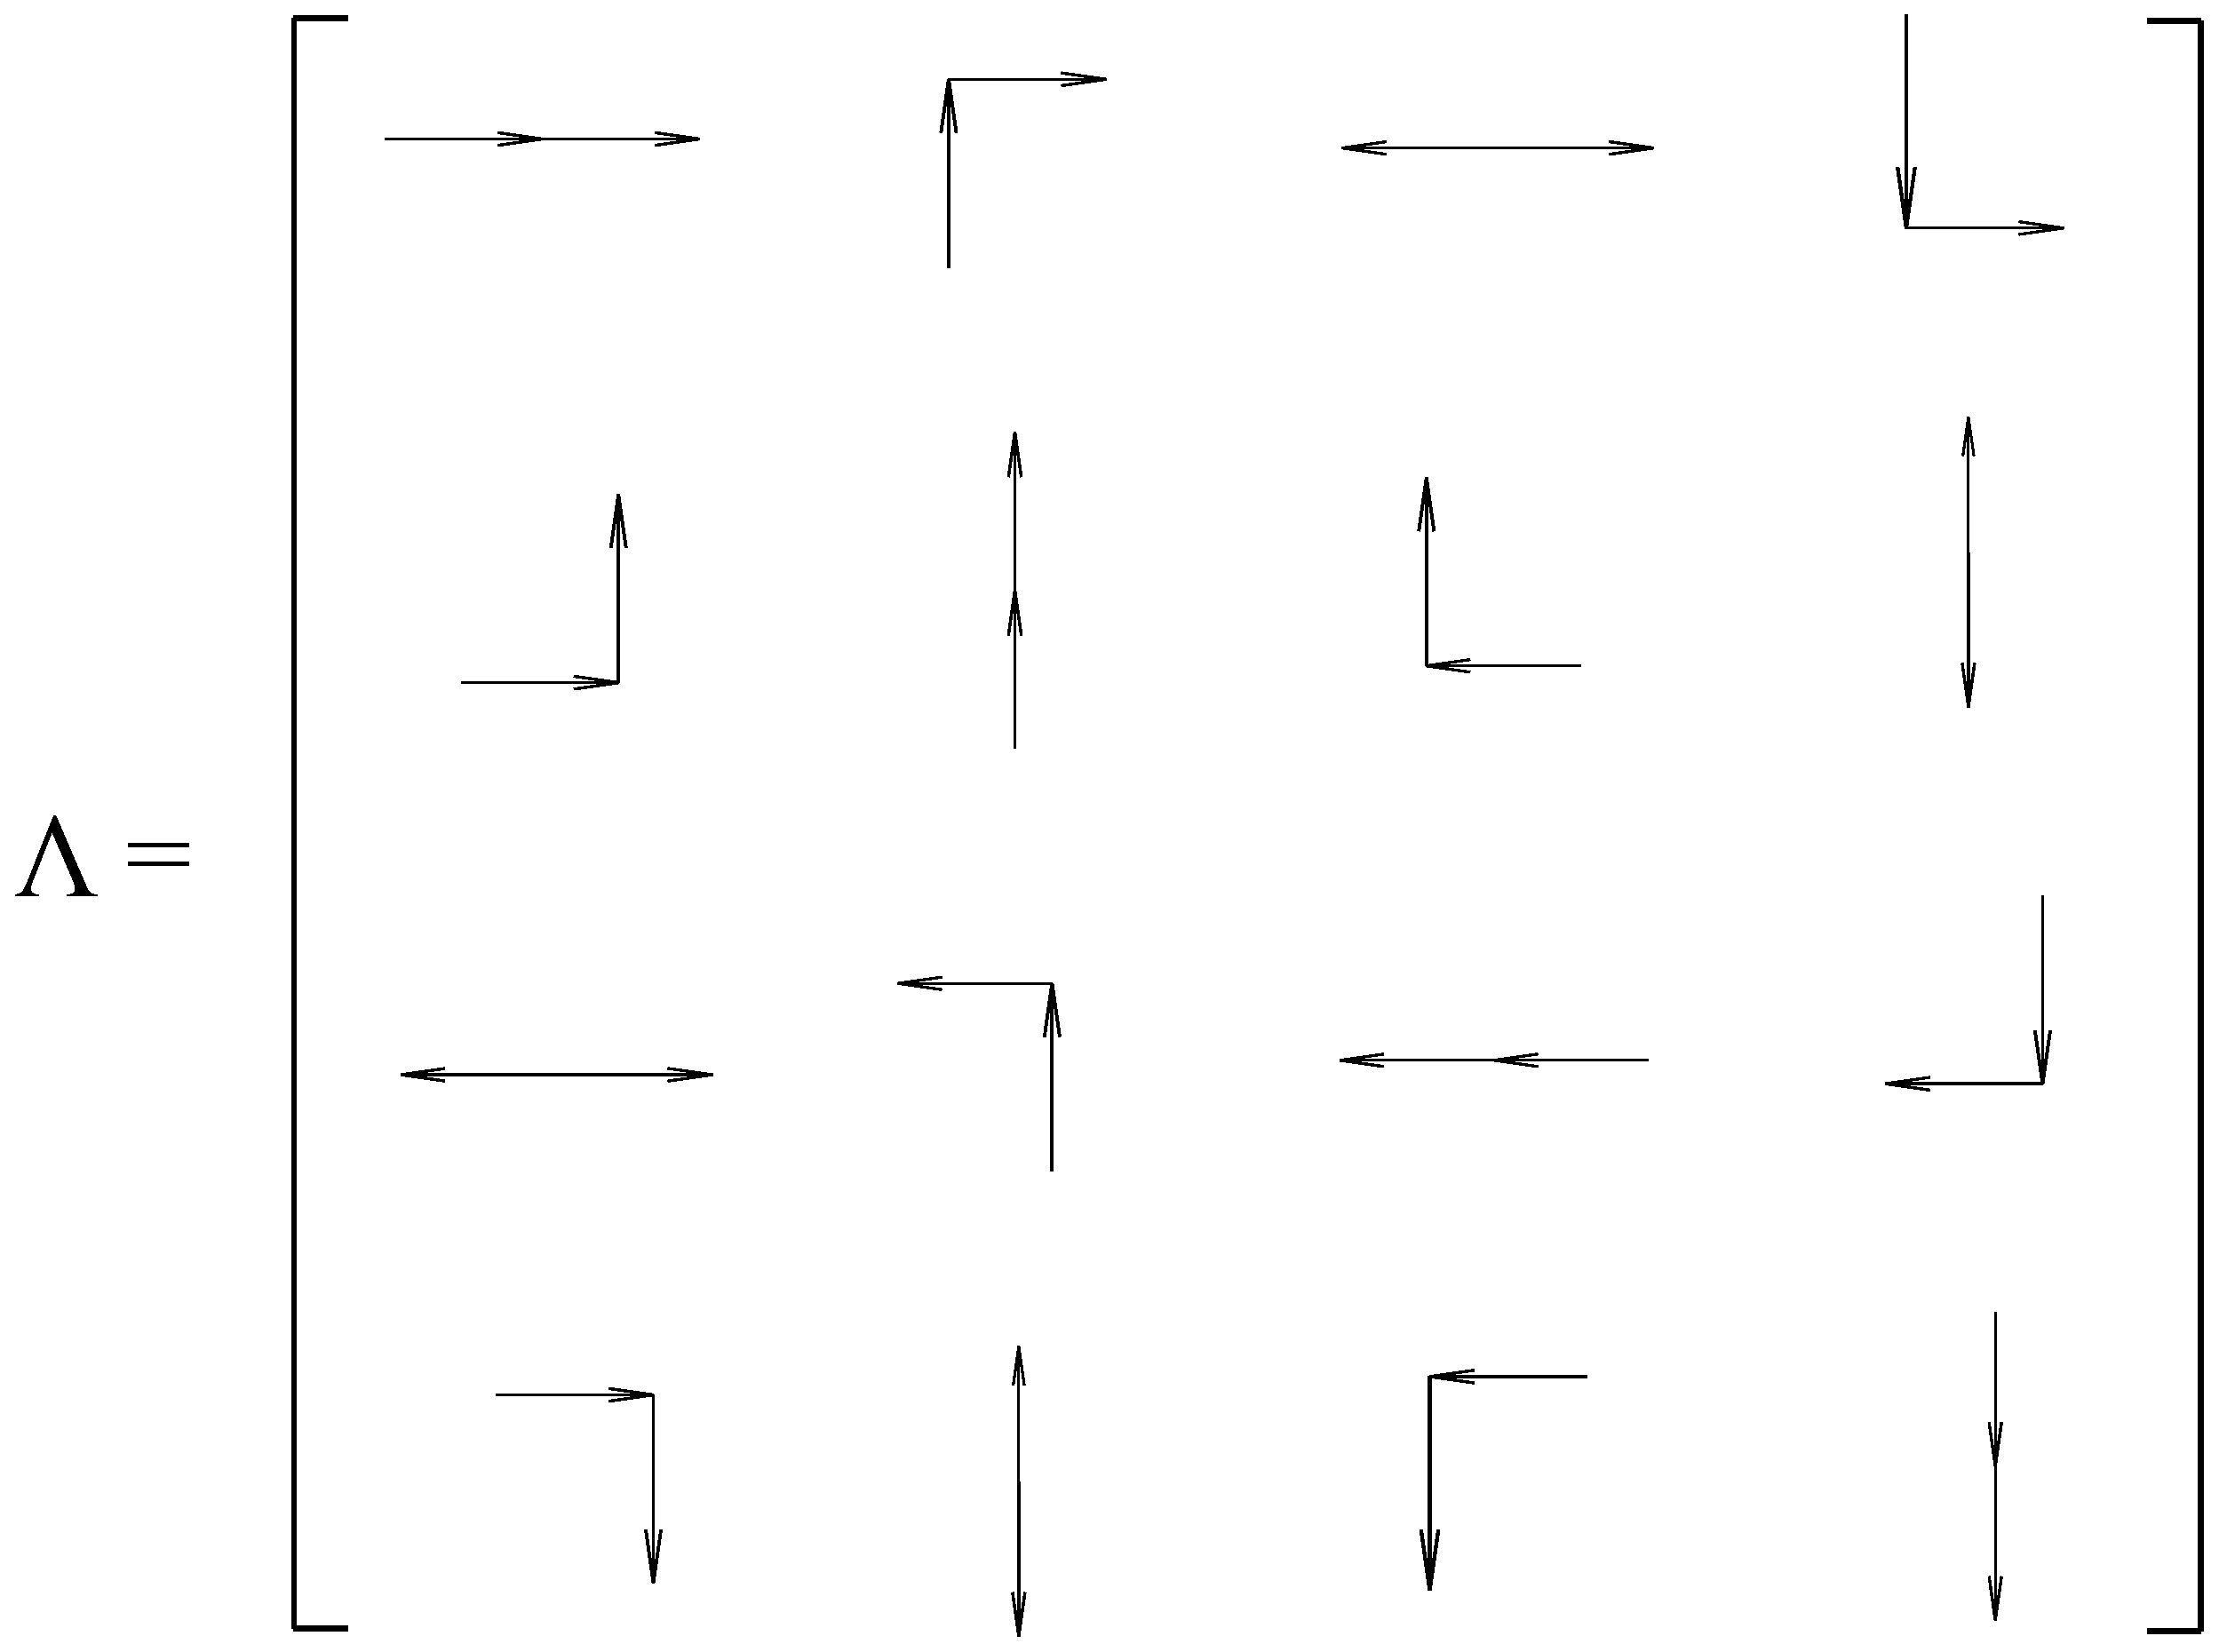
\includegraphics[width=0.5\linewidth]{part1/matrixElemSquare.eps}}
 	\caption{Элементы матрицы $\Lambda$}
 	\label{matrixElemSquare}
 \end{figure}

В свете приведенной выше интерпретации рекурсивных уравнений вероятность перехода относительно пути полной длины $r$ выражается матрицей $\Lambda^r$. Обратите внимание, что диагональные элементы этой матрицы выражают вероятность вернуться в исходную точку после прохождения цикла длины $r$, т.е. они совпадают с $W_r (i_0, j_0, \mu_0)$. Следовательно, имеем 
\begin{equation}
\Sp \Lambda^r = \sum_{i_0, j_0, \mu} W_r (i_0, j_0, \mu),
\end{equation}
и, сравнивая с \eqref{fl}, приходим к
\begin{equation}
f_r = \frac{1}{2r} \Sp \Lambda^r = \frac{1}{2r} \sum_a \lambda_a^r,
\end{equation}
где $\lambda_a$ - собственные значения матрицы $\Lambda$. Используя это выражение в \eqref{Phi} и меняя местами индексы суммы, получаем
\begin{multline}
\Phi(v) = \exp{\bigg[-\frac{1}{2}\sum_i \sum_{r=1}\frac{1}{r} v^r \lambda_i^r\bigg]} = \\ = \exp{\bigg[\frac{1}{2}\sum_i \ln(1 -  v\lambda_i)\bigg]} = \prod_i \sqrt{1 - v\lambda_i}.
\end{multline}

Последнее, что нужно сделать --- это определить собственные значения $\Lambda$. Диагонализация этой матрицы по координатам $k$ и $l$ решетки может быть легко выполнена с помощью преобразования Фурье. Фактически, определяя
\begin{equation}
W_r (p, q, \mu) = \sum_{k,l = 0} e^{-\frac{2\pi i}{L}(pk + ql)} W_r (k, l, \mu),
\end{equation}
с $N = L^2$ и преобразованием Фурье  имеем
\begin{align*}
&W_{r+1} (p, q, 1) = \epsilon^{-p}\; W_r (p, q, 1) + \epsilon^{-q} \alpha^{-1}\;  W_r (p, q, 2) + \epsilon^{q} \alpha\; W_r (p, q, 4),\\
&W_{r+1} (p, q, 2) = \epsilon^{-p} \alpha\; W_r (p, q, 1) + \epsilon^{-q}\; W_r (p, q, 2) + \epsilon^{p} \alpha^{-1}\; W_r (p, q, 3),\\
& W_{r+1} (p, q, 3) = \epsilon^{-q} \alpha\; W_r (p, q, 2) + \epsilon^{p}\; W_r (p, q, 3) + \epsilon^{q} \alpha^{-1}\; W_r (p, q, 4),\\
& W_{r+1} (p, q, 4) = \epsilon^{-p} \alpha^{-1}\; W_r (p, q, 1) + \epsilon^{p} \alpha\; W_r (p, q, 3) + \epsilon^{q}\; W_r (p, q, 4),
\end{align*}
где $\epsilon = e^{2\pi i/L}$ и $\alpha = e^{i\pi/4}$.

Поскольку $W_r (p, q, \mu)$ появляется с одинаковыми индексами $p$ и $q$ как в левой, так и в правой частях этих уравнений, преобразование Фурье матрицы $\Lambda$ диагонально по этим индексам, и мы имеем
\begin{equation}
\Lambda (p, q, \mu\; |\; p, q, \mu^{'}) = 
\begin{pmatrix}
\epsilon^{-p} & \alpha^{-1}\epsilon^{-q} & 0 & \alpha \epsilon^{q}  \\
\alpha \epsilon^{-p} & \epsilon^{-q} & \alpha^{-1}\epsilon^{p} & 0 \\
0 & \alpha\epsilon^{-q} & \epsilon^{p} & \alpha^{-1} \epsilon^{q}  \\
\alpha^{-1} \epsilon^{-p} & 0 & \alpha \epsilon^{p} & \epsilon^{q}  \\
\end{pmatrix}.
\end{equation}

Несложное вычисление показывает, что
\begin{multline}
\prod_i (1 - v\lambda_i) = \Det(I - \Lambda) = \\ = (1 + v^2)^2 - 2v (1 - v^2) \bigg(\!\!\cos \frac{2 \pi p}{L} + \cos \frac{2 \pi q}{L}\bigg),
\end{multline}
где $I$ --- единичная матрица размером $4 \times 4$.

Возвращаясь к выражению \eqref{zn2}, имеем
\begin{equation}
Z_{N} = 2^N (\ch K)^{2N} \prod_{p, q}^{L} \bigg[ (1 + v^2)^2 - 2v (1 - v^2) \bigg(\!\!\cos \frac{2 \pi p}{L} + \cos \frac{2 \pi q}{L}\bigg) \bigg]^{1/2}.
\end{equation}

Прологарифмировав обе части уравнения, получаем
\begin{multline}
\ln Z_N = N\ln 2 + 2N\ln (\ch K) + \frac{1}{2} \sum_{p,q = 0}^{L} \ln \bigg[ (1 + v^2)^2 - \\ - 2v (1 - v^2) \bigg(\!\!\cos \frac{2 \pi p}{L} + \cos \frac{2 \pi q}{L}\bigg) \bigg]. 
\end{multline}

Введем обозначения $\omega_1 = 2 \pi p / L$ и $\omega_2 = 2 \pi q /L$, также, при $L \rightarrow \infty$ сумма становится интегралом 
\begin{multline}
\ln \frac{\lambda_s}{2} = 2\ln (\ch K) + \frac{1}{8 \pi^2} \int_{0}^{2\pi} \int_{0}^{2\pi} \ln \big[ (1 + v^2)^2 - \\ - 2v (1 - v^2) (\cos \omega_1 + \cos \omega_2) \big] d \omega_1 d \omega_2.
\end{multline}

Учитывая, что $v = \th K$, после всех упрощений окончательно получаем выражение для статистической суммы (приходящейся на один узел) изотропной ($K_1 = K_2 = K $) квадратной решетки
\begin{equation}
\ln \frac{\lambda_s}{2} = \frac{1}{8 \pi^2} \int_{0}^{2\pi} \int_{0}^{2\pi} \ln \big[ \ch^2 2K - \sh 2K( \cos \omega_1 + \cos \omega_2)\big] d \omega_1 d \omega_2,
\end{equation} 
где $K = J/T$. 

Можно показать, что матрица коэффициентов $\Lambda$ для неизотропной решетки ($K_1 \neq K_2$) статсуммы \eqref{zn1} записывается в следующем виде
\begin{equation}
\Lambda (p, q, \mu\; |\; p, q, \mu^{'}) = 
\begin{pmatrix}
v\epsilon^{-p} & w\alpha^{-1}\epsilon^{-q} & 0 & w\alpha \epsilon^{q}  \\
v\alpha \epsilon^{-p} & w\epsilon^{-q} & v\alpha^{-1}\epsilon^{p} & 0 \\
0 & w\alpha\epsilon^{-q} & v\epsilon^{p} & w\alpha^{-1} \epsilon^{q}  \\
v\alpha^{-1} \epsilon^{-p} & 0 & v\alpha \epsilon^{p} & w\epsilon^{q}  \\
\end{pmatrix}.
\end{equation}

Вычисляя определитель этой матрицы, получаем 
\begin{multline}
\prod_i (1 - \lambda_i) = \Det(I - \Lambda) = (1 + v^2)(1 + w^2) -\\- 2w (1 - v^2) \cos \frac{2 \pi p}{L}-  2v (1 - w^2) \cos \frac{2 \pi q}{L}.
\end{multline}

Тогда статсумма \eqref{zn1} может быть записана в форме
\begin{multline}
Z_{N} = 2^N (\ch K_1 \ch K_2 )^N \prod_{p, q}^{L} \bigg[ (1 + v^2)(1 + w^2) -\\- 2w (1 - v^2) \cos \frac{2 \pi p}{L}- 2v (1 - w^2) \cos \frac{2 \pi q}{L} \bigg]^{1/2}.
\end{multline}

При $v = \th K_1$ и $w = \th K_2$ приходим к окончательному выражению для статистической суммы (приходящейся на один узел) обычной квадратной решетки
\begin{equation}
\ln \frac{\lambda_s}{2} = \frac{1}{8 \pi^2} \int_{0}^{2\pi} \int_{0}^{2\pi} \ln \big[ \ch 2K_1 \ch 2K_2 - \sh 2K_1 \cos \omega_1 - \sh 2K_2 \cos \omega_2\big] d \omega_1 d \omega_2,
\end{equation} 
($K_1 = J/T$, $K_2 = J^{'}/T)$.


\section{Понятие декорированной решетки} 

В современной физике конденсированного состояния активно исследуются модели магнитных материалов, в которых кроме обменных взаимодействий учитываются разные усложняющие факторы, не учитываемые моделями первого приближения. Данные факторы позволяют оказывать значительное влияние на характер критического поведения магнетиков и приводить к существованию большого разнообразия магнитных упорядоченных состояний и фазовых переходов между ними. За последнее время значительно возрос интерес к исследованию декорированных структур.

\begin{figure}[h]
	\center{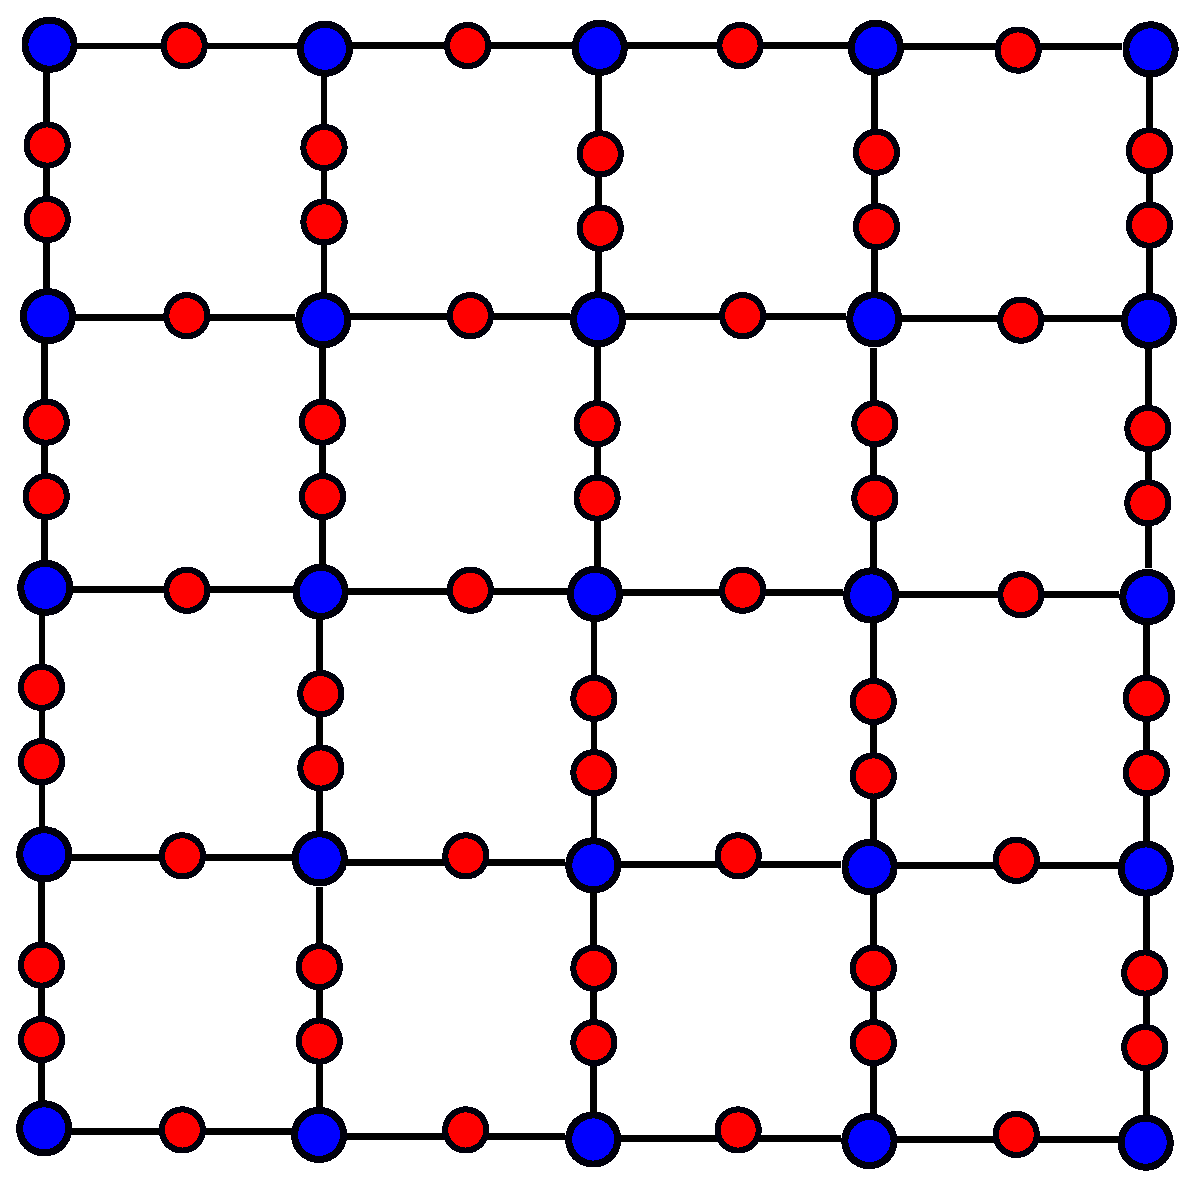
\includegraphics[width=0.6\linewidth]{part1/decorSquare.eps}}
	\caption{Декорированная квадратная решетка (единожды декорирована в горизонтальном направлении и дважды декорирована в вертикальном направлении). Синим цветом обозначены нодальные спины, красным --- декорационные спины}
	\label{decorSquare}
\end{figure}

Термин \guillemotleft декорированная решетка\guillemotright \hspace{1pt} был введен в работе Сиози~\cite{siozi1951}, после чего данная концепция начала стремительно развиваться другими авторами~\cite{siozi_domb1972, fisher1958}. Изучение данной области уже довольно богато литературой (см., например,~\cite{jaščur2016, strečka2019_1, strečka2019_2, gálisová2018, cenčariková2016, stubňa2017, mutalamov2020}). Это можно объяснить тем, что декорирование порождает ряд новых, еще не до конца изученных эффектов по сравнению с исходными недекорированными решетками. В частности, декорирование порождает многообразие различных фрустрационных эффектов, может приводить как к подавлению фазовых переходов, присущих недекорированным решеткам, так и к возникновению новых фазовых переходов. Вместе с тем, появляются новые типы частичного упорядочения, а также различные формы расщепления теплоемкости. Богатство критического поведения декорированных решеток обусловлено возможностью многократного декорирования.

\begin{figure}[h]
	\center{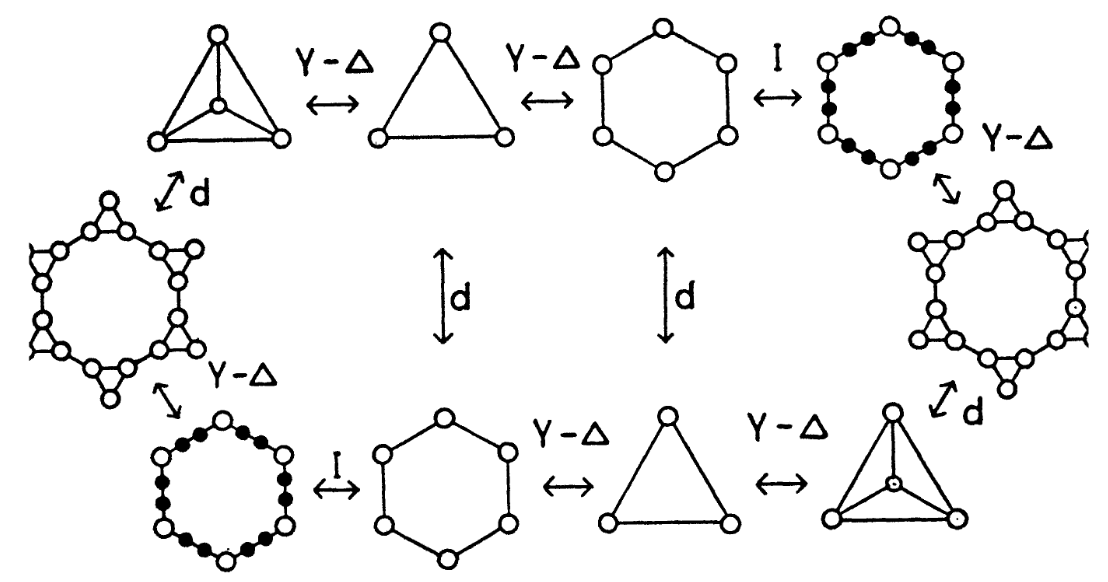
\includegraphics[width=1\linewidth]{part1/transformCycle.png}}
	\caption{Циклическое преобразование решеток: $d$ --- дуальное преобразование, $Y - \Delta$ --- преобразование \guillemotleft звезда-треугольник\guillemotright \hspace{1pt}, $I$ --- декорационное преобразование~\cite{siozi_domb1972}}
	\label{transformCycle}
\end{figure}

Суть построения декорированной решетки заключается во введении дополнительных спинов в промежутки между узлами исходной решетки~\cite{siozi_domb1972}. Данную процедуру можно реализовывать и в обратном порядке, превращая декорированные решетки в обычные. Основные спины еще называют нодальными, а дополнительные спины --- декорационными (рисунок \ref{decorSquare}). Практически большинство реальных структур является декорированными.

Стоит отметить, что точного аналитического решения модели Изинга на декорированной решетке в магнитном поле до настоящего момента получено не было~\cite{kassan-ogly2019, proshkin2019, kassan-ogly2020}. И только в настоящей работе мы приводим впервые полученное точное решение модели Изинга на декорированной решетке при наличии магнитного поля~[A3].

Напоследок, следует обратить внимание, что, наряду с дуальным преобразованием (преобразование обычной решетки в решетку к ней дуальную, которое идет посредством помещения в центр ячейки исходной решетки узла, после чего эти узлы соединяются, образуя дуальную решетку) и преобразованием \guillemotleft звезда-треугольник\guillemotright \hspace{1pt}, декорационное преобразование является важной процедурой при переходе от одной решетки к решетке совершенно иной топологии (рисунок \ref{transformCycle}).

\section{Постановка задачи исследования}

Цель настоящей кандидатской диссертации заключается в рассмотрении обобщенной модели Изинга с различными обменными взаимодействиями как между ближайшими, так и между вторыми соседями на одномерной цепочке с учетом декорирования и магнитного поля, а также на декорированных двумерных решетках, но в отсутствие поля, с последующим изучением их термодинамических, магнитных и фрустрационных свойств.

Для достижения цели были поставлены следующие задачи:
\begin{enumerate}
    \item Получить точное аналитическое решение обобщенной модели Изинга на одномерной цепочке при учете магнитного поля методом трансфер-матрицы Крамерса--Ваннье.
    \item Исследовать термодинамические, магнитные и фрустрационные свойства обобщенной модели Изинга на одномерной цепочке, в том числе при учете декорирования.
    \item Получить точное аналитическое решение обобщенной модели Изинга на квадратной решетке комбинаторным методом Вдовиченко--Фейнмана.
    \item Исследовать термодинамические и фрустрационные свойства обобщенной модели Изинга на квадратной решетке.
\end{enumerate}

\FloatBarrier
